
\documentclass[12pt, a4paper, english, brazil]{article}

% Sistema autor-data com títulos nas referências em negrito
% \usepackage[alf,abnt-emphasize=bf]{abntex2cite}

% \usepackage[alf,abnt-emphasize=bf,abnt-repeated-author-omit=yes,abnt-year-extra-label=yes]{abntex2cite}	% Citações padrão ABNT

% ----------------- link in the PDF
% http://tug.ctan.org/macros/latex/contrib/abntex2/doc/abntex2cite.pdf
%Usando o pacote abntex2cite autonomamente ... é preciso passar a opção carregando o pacote url antes do abntex2cite
\usepackage[hyphens]{url}
\usepackage[bookmarks=false]{hyperref}
\usepackage{hyperref}
% ----------------- link in the PDF

\usepackage[alf,abnt-emphasize=bf,abnt-repeated-author-omit=yes]{abntex2cite}

\usepackage[utf8]{inputenc}	
\usepackage[brazil]{babel}
\usepackage{graphicx,url}
\usepackage{subfigure}
\usepackage{enumitem}
\usepackage{amsfonts}
\usepackage{amsmath}

\usepackage{physics}
\usepackage{comment}

\usepackage{lscape}

\usepackage{fancyhdr}
\usepackage[all]{hypcap}    %for going to the top of an image when a figure reference is clicked

\usepackage{booktabs}
\usepackage{multirow}

% -
\usepackage{indentfirst}
% \graphicspath{{img/}}
%\pagestyle{empty}

\usepackage{xcolor}

\newcommand{\textRed}[1]{{{\color{red} #1}}}
\newcommand{\textBlue}[1]{{{\color{blue} #1}}}
\newcommand{\dotsBlue}{\colorbox{orange}{\textcolor{blue}{\dots}}}
\newcommand{\boxRed}[1]{\colorbox{red}{#1}}
\newcommand{\boxYellow}[1]{\colorbox{yellow}{#1}}
\newcommand{\linePage}{--------------------------------------------------------------------------------------------------------------}

\usepackage{tabularx}
\newcolumntype{L}{>{\raggedright\arraybackslash}X}
\usepackage{amssymb}% \varnothing

% -

\textwidth 16cm \textheight 23.2cm
\voffset -1.5cm \hoffset -1.4cm

\sloppy

\begin{document}

\rhead{\thepage}
\pagenumbering{arabic}

\begin{center}
	\bf{\LARGE{PROJETO DE DISSERTAÇÃO}\\ $\ $\\}
	\Large{Programa de Mestrado em Ciência da Computação\\
		Universidade Federal de Uberlândia}\\ $\ $\\
\end{center}

\begin{center}
	\bf{Aluno: João Batista Ribeiro\\ $\ $\\
		Orientador: Prof. Dr. André Ricardo Backes\\ $\ $\\
		Coorientador: Prof. Dr. Maurício Cunha Escarpinati\\ $\ $\\
		Data da formalização da coorientação no colegiado: \colorbox{yellow}{xx/xx/2021}\\ $\ $\\
		Título do Trabalho: \colorbox{yellow}{Detecção de linhas de plantio em plantações de cana-de-açúcar}\\ $\ $\\
		Data de Início como Aluno Regular: março de 2021\\ $\ $\\
		Previsão da Defesa: fevereiro de 2023\\ $\ $\\}
\end{center}

\textRed{Versão 3 - 01/11/2021}

\section{Introdução}

O rápido crescimento populacional, principalmente no último século, tem impulsionado a demanda por alimentos e a utilização inteligente/sustentável dos recursos naturais. Nesse contexto, a agricultura aliada tecnologia, chamada de Agricultura de Precisão (AP), busca suprir essa demanda utilizando os recursos sob medida com base nas informações coletadas. A AP engloba uma série de técnicas diferentes, como a análise espacial da área plantada, informações do solo e das plantas, permitindo aos produtores planejar e monitorar suas plantações \cite{Blasch_2020}.

A Agricultura de Precisão se tornou possível graças ao desenvolvimento e avanços de diferentes tecnologias, como o Sistema de Posicionamento Global (GPS), o uso de imagens de satélites, o desenvolvimento de novas técnicas de Processamento Digital de Imagens (PDI) e Visão Computacional, sensoriamento remoto entre outras. Isso possibilitou o desenvolvimento de metodologias, técnicas e programas que são aplicados nas várias etapas da agricultura, desde análise e preparação do solo (para determinar a escassez de determinado nutriente numa região) até a utilização de veículos autônomos para fazer a pulverização de defensivos (com quantidade específica para cada parte do talhão) e na colheita seguindo as linhas de plantio. Muitos dos avanços na AP são fortemente dependentes das tecnologias de processamento digital de imagens \cite{Bolfe_2020}.

As imagens utilizadas na AP têm variadas fontes (e.g., câmeras acopladas em Veículos Aéreos Não Tripulados (VANTs) e satélites) dependendo da aplicação e do \textit{Ground Sample Distance} (GSD) requisitado. O GSD refere-se à distância da amostra ao solo, ou seja, quanto cada pixel da imagem obtida representa da região fotografada. Assim quanto menor for o GSD, mais detalhes a imagem terá da região analisada. Satélites (com GSD em média de metros) conseguem imagem de grande regiões mais facilmente que os VANTs (GSD em média de centímetros), que necessitam de planos de voo para abranger toda região e mosaicagem para combinar as imagens obtidas \cite{Messina_2020}.

O custo das imagens de satélites depende muito da qualidade das imagens, elas possuem baixa temporalidade (imagens de uma mesma área em momentos diferentes), um baixo nível de detalhes (maior GSD) em relação aos VANTs e sofrem bastante com as condições climáticas (e.g., nuvens). Por outro lado, os VANTs geralmente têm custo baixo para aquisição das imagens, possibilitam a captura (e recaptura) das imagens sempre que necessário (alta temporalidade e disponibilidade), com grande nível de detalhes (pequeno GSD) e não sofrem muito com as nuvens devido a sua altitude de voo \cite{Candiago_2015, Delavarpour_2021}.

Uma das aplicações importantes da AP é a detecção das linhas de plantio, principalmente porque esta é utilizada como uma etapa importante para outras aplicações da AP (e.g., detecção de ervas daninhas, mapeamento e previsão de produção de safra, detecção de falhas) \cite{Hassanein_2019}. Além de ser utilizada pelos veículos autônomos para se guiarem na plantação, assim evitando o pisoteamento da cultura \cite{Doha_2021}.

A detecção de linhas de plantio é uma tarefa complexa e com vários desafios. Por exemplo, pode haver a presença de ervas daninhas com assinatura espectral e cor semelhantes a linhas da cultura, dificultando a sua detecção. Crescimento irregular da cultura, falhas no plantio, imperfeições e oclusões linha de plantio, manchas de solo e tipos diferentes na mesma plantação, presença de artefatos bloqueando a visão da linha de cultivo (e.g., árvores), sombras, além de variações nas condições climáticas e de iluminação, são exemplos de variações presentes nas imagens e que podem atrapalhar, ou mesmo comprometer, o processo de detecção  \cite{Rabab_2021, Doha_2021}.

Um dos cenários de grande utilização da Agricultura de Precisão no Brasil é no cultivo de cana-de-açúcar (\textit{Saccharum officinarum}), motivando pesquisadores (e.g., \citeonline{Souza_2017, Souza_2018, Silva_Escarpinati_Backes_2021}) e empresas (e.g., \citeonline{AERO_2017, Sensix_2020, Inforow_2021}) a desenvolverem soluções na área.

O Brasil é o maior produtor e exportador de cana-de-açúcar, com aproximadamente 10 milhões de hectares de área plantada, sendo que mundialmente esse valor é de pouco mais de 26 milhões de hectares \cite{Ritchie_2020, IBGE_2021, FAOSTAT_2021}. O seu cultivo é de grande importância para a economia brasileira devido as suas diversas aplicações. A cana-de-açúcar pode, por exemplo, ser consumida fresca na alimentação humana e forragem na alimentação animal, produção de açúcar, bebidas, energia e combustíveis. Além disso, seus subprodutos, como o bagaço e a palha, podem ser utilizados na fertilização do solo \cite{Oliveira_2018}.

A cana-de-açúcar é uma cultura semi-perene (seu manejo pode durar anos sem ser necessário um novo plantio), o que adiciona uma motivação a mais para detectar as suas linhas de plantio em relação a outras culturas (e.g., milho). Após a primeira colheira, a rebrota das soqueiras é colhida anualmente por cerca de 5 a 7 anos, ou mais \cite{Rudorff_2010}. Contudo, isso também adiciona um desafio, pois dependendo do estágio da plantação, folhas secas estão presentes no solo entre as linhas da cultura, dificultando a análise computacional \cite{Silva_2020}.

Apesar de na literatura já existirem muitos trabalhos para detectar linhas de plantio, a maioria deles são para outras culturas (e.g., milho e beterraba) ou focados em linhas retas \cite{Pereira_Junior_2020}. Além de muitos utilizarem imagens de baixíssima altitude ($\le$ 2 m), tiradas a partir do solo (manualmente ou acopladas no maquinário agrícola) ou de alta altitude (imagens de satélites) \cite{Hasan_2021}.

Outro ponto importante, atualmente não é possível encontrar nenhum \textit{software} gratuito e de código aberto que faça a detecção das linhas de plantio corretamente (em cana-de-açúcar ou outro tipo de cultura), apenas \textit{softwares} comerciais, como o \citeonline{Inforow_2021}. Assim este projeto também busca desenvolver uma metodologia de detecção das linhas de plantio que possa ser utilizada no desenvolvimento de um \textit{software}, promovendo uma democratização do conhecimento.

Considerando o cenário de grande utilização dos VANTs para obtenção de imagens para a Agricultura de precisão, a grande importância da detecção das linhas de plantio, este projeto tem como foco a detecção de linhas de plantio de cana-de-açúcar.

%\subsection{Motivação}
    % Deixar dentro da introdução
 
\subsection{Objetivos}

    % => Descreva claramente os desafios que o tema propõe e quais os objetivos que se pretende alcançar. Se o tema for muito abrangente, descreva os objetivos em termos de ``objetivo geral'' e ``objetivos específicos''. Cuidado com objetivos como ``desenvolver um sistema...''; ``explorar um método...'' Esses objetivos são triviais, ou seja, uma vez desenvolvido o sistema ou explorado o método, independente dos resultados, o objetivo foi atingido. Prefira verbos como: ``contribuir'', ``analisar'', ``investigar'', ``comparar''. Os membros da banca ao lerem essa seção farão o seguinte questionamento: Algum conhecimento novo para a humanidade foi produzido?

Este projeto tem como objetivo principal estudar e analisar os diferentes métodos de segmentação automática em imagens de VANTs tendo, inicialmente, foco em imagens de plantio de cana-de-açúcar e propor melhorias na detecção de linhas de plantio. 
Este projeto tem como objetivos específicos:

\begin{itemize}
    \item Estudar e analisar os métodos propostos na literatura correlata para detecção das linhas de plantio, como por exemplo, transformada de Hough e Radon, segmentação, redes neurais convolucionais, índices de vegetação e operações morfológicas.

    \item Avaliar a detecção de linhas de plantio utilizando as imagens de VANTs em métodos de \textit{Deep Learning} juntamente com Índice de Vegetação.

    \item Detectar as linhas de plantio nas imagens das plantações de cana-de-açúcar, com plantas em variados estágios (antes do primeiro corte (cana-planta) e depois do primeiro corte (cana-soca)).

    \item Desenvolver um método capaz de identificar, nas imagens obtidas por VANTs, as linhas de plantio com formatos de linhas retas e linhas curvas.

    \item Aplicar a proposta em imagem reais de plantações de cana-de-açúcar, analisar e avaliar os resultados provenientes das melhorias com ajuda de especialistas.
\end{itemize}

% \subsection{Hipótese} 
    % => Descreva claramente quais são as hipóteses da sua pesquisa (Uma hipótese é uma suposição para a solução do problema que você pretende desenvolver). Indique quais perguntas estão associadas a sua hipótese. Lembre-se que as hipóteses deverão ser comprovadas via os experimentos propostos na seção que descreve o método de pesquisa.
% => colocar nos objetivos

%\subsection{Contribuições}
    % => Liste as contribuições do seu trabalho. 

\section{Revisão da literatura correlata}
    % => Descreva os principais trabalhos existentes na literatura da área que estão relacionados com o trabalho que você está propondo e deixe claro qual a sua contribuição em relação a estes trabalhos. O que você está propondo de novo que estes trabalhos não abordaram ou abordaram de forma ineficiente? Eventualmente, se for o caso, introduza nesta seção os conceitos teóricos existentes na literatura que são necessários para a descrição de seu projeto de tese.

Esta seção apresentará os principais conceitos utilizados neste projeto, bem como alguns trabalhos relacionados.

\subsection{Processamento digital de imagens}

O Processamento Digital de Imagens (PDI) compreende a manipulação de imagens digitais por um computador de modo a atingir um objetivo específico com procedimentos envolvendo varias etapas \cite{Gonzalez_Woods_2010}.

Após a aquisição das imagens, é comum utilizar uma etapa de pré-processamento das imagens, onde são feitos ajustes na intensidade dos pixels (sem conhecimento sobre o que representam). Esses ajustes visam remover imperfeições (e.g., presença de pixels ruidosos, contraste e/ou brilho inadequado) geradas no processo de aquisição e realçar detalhes importantes para análise. Assim, essa etapa tem como objetivo melhorar a imagem original para ser utilizada no processamento principal \cite{Marques_Filho_1999}.

Dependendo do contexto da aplicação, muitas são as técnicas de pré-processamento que podem ser utilizadas, dentre elas a correção de brilho e contraste, realce de brilho, realce de bordas. A seguir são descritas em detalhes algumas dessas etapas.

\subsubsection{Segmentação}

A segmentação de imagens tem como objetivo dividir a imagem em regiões ou objetos de interesse. O nível de divisões depende do problema a ser resolvido, sendo a segmentação executada até que todos os objetos de interesse sejam detectados. A segmentação de imagens é considerada uma das tarefas mais difíceis do PDI, já que implica diretamente no resultado da etapa de análise. Assim, é importante selecionar qual a técnica de segmentação mais adequada para o seu problema, de modo a aumentar a probabilidade de se obter uma segmentação precisa \cite{Gonzalez_Woods_2010}.

Ao fim da etapa de segmentação a imagem é dividida em várias regiões e sem sobreposição entre elas, ou seja, uma parte da imagem pertence somente a uma região de interesse. O tipo de segmentação utilizada depende do problema a ser tratado, por exemplo, se for necessário dividir a imagem em regiões sem rotular elas (segmentação clássica), ou se for necessário rotular cada pixel da imagem a uma determinada classe (segmentação semântica). Dentre as técnicas de segmentação, a limiarização é uma das mais utilizadas, por ser eficiente e simples do ponto de vista computacional \cite{Kuruvilla_2016}.

Uma forma bastante simples de segmentação é a limiarização (\textit{Thresholding}, em inglês), que consiste na divisão da imagem em duas classes (fundo e objeto) a partir de um limiar $T$. Caso o valor do pixel seja maior ou igual a $T$, esse terá valor 1 na imagem gerada; caso contrário, este receberá o valor 0. Como resultado, esse processo produzirá uma imagem binária (com pixels de valor 0 ou 1), processo também chamado de binarização \cite{Marques_Filho_1999}.

A escolha do limiar é uma tarefa complicada já que um limiar inadequado não conseguirá separar de forma correta a imagem em duas classes. Nesse contexto, a aplicação de limiares locais (i.e., um para cada pequeno retângulo da imagem de modo a compensar a não uniformidade de iluminação e/ou a refletância), pode ser uma opção melhor. Outra abordagem é a utilização de múltiplos limiares globais, onde a imagem é divida em função dos intervalos dos limiares em mais de duas classes \cite{Gonzalez_Woods_2010}.

O limiar pode ser escolhido manualmente ou através do uso de algum algoritmo. Para a escolha desse limiar muitos trabalhos na área de imagens utilizam o método de Otsu. Este método \cite{Otsu_1979} utiliza o histograma da imagem e busca um limiar ideal que separe a imagem em duas classes (objeto e fundo), de modo a maximizar a variância entre as classes e minimizar a variância interna das classes.

\subsubsection{Transformada de hough}

A Transformada de Hough (TH) é um método desenvolvido, inicialmente, para detectar linhas retas em imagens binárias, que depois foi expandido para a detecção de formas parametrizadas (e.g., círculos e elipses). A transformada tem por base um método de votação (acumulador) do espaço da imagem (pixels) para o espaço de parâmetros, chamado de espaço de Hough. Nele, as coordenadas polares geralmente são preferidas, pois podem ser limitadas em intervalos muito precisos, ao contrário das coordenadas cartesianas \cite{Bah_2020}.

Uma linha reta em uma imagem é composta por um conjunto de pixels, onde pela TH é mapeada para um único ponto $(\rho, \theta)$ no espaço de Hough, de acordo com a equação da reta, $\rho = x \cos \theta + y \sin \theta$, onde $\rho$ representa a distância da reta até a origem e $\theta$ representa o ângulo entre o eixo $x$ e a reta (\autoref{fig:tHough}). A TH é capaz de detectar que um conjunto de pixels pertencem a uma linha reta mesmo que a reta esteja descontinua (faltando alguns pixels) e/ou com ruídos. Deste modo, todos os pontos alvo $(x, y)$ da imagem binária após a execução da TH terão seus respectivos ($\rho, \theta$), sendo acumulados caso coincidirem, ou seja, serem pontos colineares \cite{Huiying_2015}.

\begin{figure}[ht]
    \centering
    \subfigure[]{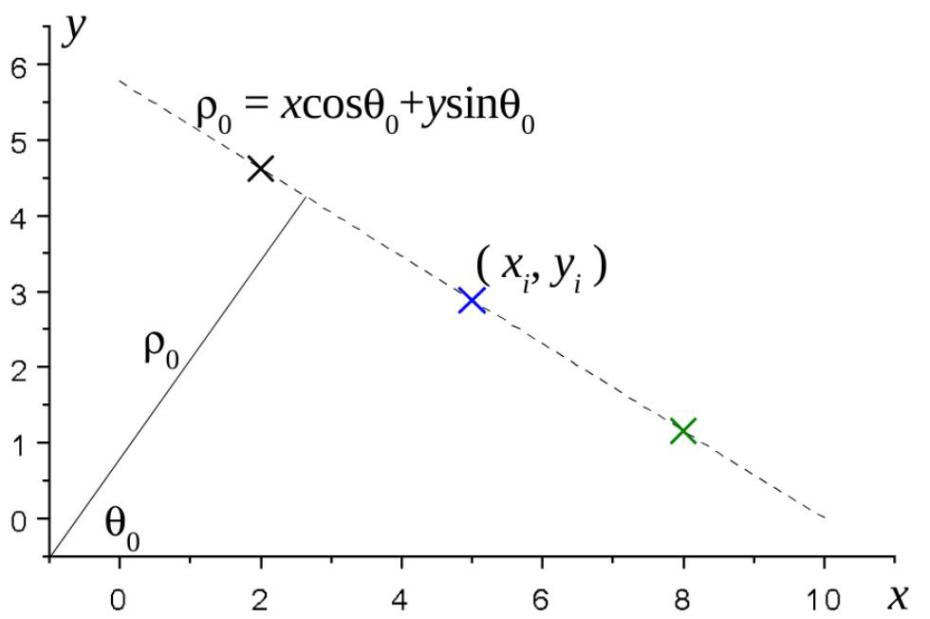
\includegraphics[width=0.45\textwidth]{img/ht_a.jpg}}
    \subfigure[]{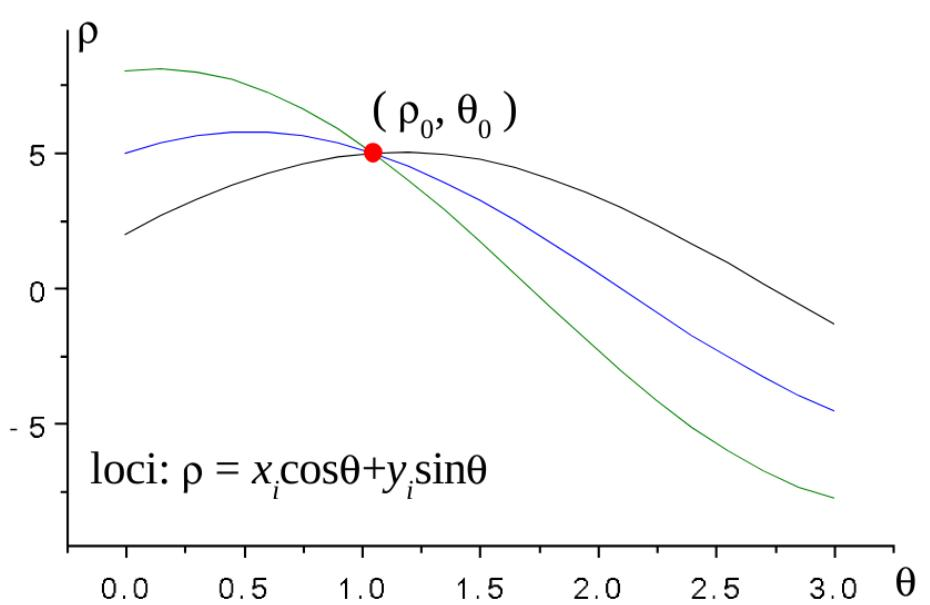
\includegraphics[width=0.45\textwidth]{img/ht_b.jpg}}
    \caption{Tranformada de Hough em uma linha reta: (a) espaço de entrada $(x,y)$; (b) espaço de Hough $(\rho, \theta)$ \cite{Lin_Otobe_2001}.}
    \label{fig:tHough}
\end{figure}

\subsubsection{Transformada de radon}

A Transformada de Radon (TR), proposta por Johann Radon em 1917, mapeia uma função de coordenadas cartesianas $(x, y)$ para distância e espaço angular $(\rho, \theta)$, i.e., para o domínio de Radon. Aplicada em uma imagem, ela calcula as projeções dos dados ao longo dos ângulos especificados. O conjunto dessas projeções é chamado de sinograma. A TR é útil para detectar características lineares em uma imagem, onde transforma uma linha de pixel em um único ponto \cite{Kaur_Sahambi_2015}. É matematicamente definida como:

\begin{equation}
R(\rho, \theta) = \int\limits _{-\infty}^\infty \int\limits _{-\infty}^\infty i (x, y) \delta (\rho - x\cos \theta - y\sin \theta ) dxdy
\end{equation}

onde $i (x, y)$ representa a função ou imagem em que a transformada foi aplicada, $\delta$ é o Delta de Dirac e $(\rho - x\cos \theta - y\sin \theta)$ é a equação da linha. Assim, a transformada de Radon em uma imagem pode ser definida como uma série de integrais de linha por meio de $i (x, y)$ em deslocamentos diferentes da origem \cite{Li_2019}. A TR é muito importante em diversas áreas, principalmente no processamento de imagens, sendo a base para a tomografia computadorizada clássica \cite{Silva_Escarpinati_Backes_2021}.

\subsubsection{Operações morfológicas}

A expressão morfologia é comumente utilizada no ramo da biologia para se referir ao estudo das formas e estruturas dos animais e das plantas. No contexto de processamento de imagens, a morfologia matemática tem sentido similar, sendo utilizada para extrair componentes das imagens que são úteis na representação e na descrição da forma de uma região. A morfologia matemática oferece operações úteis para resolver vários problemas de PDI, como a detecção de bordas, a segmentação e o realces de objetos presentes na imagem \cite{Marques_Filho_1999}.

A morfologia matemática utiliza a teoria dos conjuntos, onde os conjuntos representam objetos presentes na imagem. Em imagens binárias, os conjuntos são membros do espaço inteiro bidimensional $Z^2$ (onde cada elemento é um vetor de coordenadas $(x, y)$), já em imagem em escala de cinza os elementos são membros do $Z^3$, sendo os dois primeiros as coordenadas do pixel e o terceiro, seu nível de cinza \cite{Gonzalez_Woods_2010}.

As operações morfológicas utilizam os chamados elementos os estruturantes (pequenos conjuntos ou subimagens) e as operações de conjunto (e.g., a reflexão e a translação) como base. A translação é definida pela \autoref{equa:translacao}, onde os pontos em B, com as coordenadas $(x, y)$ foram substituídas por $(-x, -y)$. Por outro lado, a reflexão é definida pela \autoref{equa:reflexao}, onde os pontos em $B$, com as coordenadas $(x, y)$ foram substituídas por
$(x + z_1, y + z_2)$ \cite{AlAzawee_2015}.

\begin{equation}
    \hat{B} = \{w | w = -b\text{, para } b \in B\}
    \label{equa:translacao}
\end{equation}

\begin{equation}
    (B)_z = \{c | c = b + z\text{, para } b \in B\}
    \label{equa:reflexao}
\end{equation}

Dentre as operações morfológicas, quatro das mais utilizadas são, a dilatação, a erosão, a abertura e o fechamento. As duas primeiras são mais básicas, enquanto as duas últimas são combinações das mesmas. Considerando A e B como conjuntos de $Z^2$ e assim sendo imagens binárias. A dilatação, definida pela \autoref{equa:dilatacao}, é responsável pelo aumento ou crescimento dos limites dos objetos na imagem em função do elemento estruturante. Assim, a dilatação pode ser utilizada para preencher lacunas entre os objetos de interesse. Por outro lado, a erosão, definida pela \autoref{equa:erosao}, diminui a quantidade de pixeis de interesse em torno dos objetos dando origem à lacunas. Assim a erosão pode ser utilizada para separar objetos que estejam ligados por pequenos filamentos \cite{Marques_Filho_1999}.

\begin{equation}
    A \oplus B = \{z | (\hat{B})_z \cap A \neq \varnothing \}
    \label{equa:dilatacao}
\end{equation}

\begin{equation}
    A \ominus B = \{ z | (B)_z \subseteq A\}
    \label{equa:erosao}
\end{equation}

A aplicação de uma dilatação seguida por uma erosão (com o mesmo elemento estruturante) é definida como fechamento morfológico. Por outro lado a abertura é o oposto, uma erosão seguida de uma dilatação. A abertura e o fechamento geralmente suavizam os contornos dos objetos presentes na imagem, mas a abertura tende a quebrar trechos muito obtusos e estreitos, já o fechamento tende a frechar pequenas lacunas e preencher falhas de um contorno \cite{Gonzalez_Woods_2010, Kaur_Sahambi_2015}.

\subsubsection{Índices de vegetação}

Índices de Vegetação (IV) são combinações algébricas de várias bandas espectrais, de modo a destacar a vegetação e suas as propriedades (e.g., quantidade de biomassa, ausência de determinados nutrientes, deficiências hídricas, porcentagem de cobertura do solo) \cite{Candiago_2015}. Cada IV tem foco em certas características da vegetação e um momento mais oportuno para seu uso. Dentre eles, o índice de Excesso de Verde (do inglês \textit{Excess Green index} (ExG)) é um dos mais usados para câmeras RGB \cite{Pereira_Junior_2020}. 

Para o cálculo do índice ExG, primeiramente cada banda da imagem RGB é normalizada no intervalo de $[0, 1]$, pela \autoref{equa:normalizada}, onde $R_{max}$, $G_{max}$ e $B_{max}$ são os valores máximos correspondente de cada canal, que geralmente é 255 para imagens de 24 bits de cor. $R$, $G$ e $B$ correspondem as bandas RGB de uma imagem, R (\textit{Red} - vermelho),  G (\textit{Green} - verde) e B (\textit{Blue} - azul). Na sequência é calculado as coordenadas cromáticas, r, g e b pela \autoref{equa:chromatic}. Por fim o ExG é calculado pela \autoref{equa:exg} \cite{Garcia_2017}.

\begin{equation}
    R_n = \frac{R}{R_{max}} \text{, } G_n = \frac{G}{G_{max}} \text{, } B_n = \frac{B}{B_{max}}
    \label{equa:normalizada}
\end{equation}

\begin{equation}
    r = \frac{R_n}{R_n + G_n + B_n} \text{, } g = \frac{G_n}{R_n + G_n + B_n} \text{, } b = \frac{B_n}{R_n + G_n + B_n}, \text{ onde } r + g + b = 1
    \label{equa:chromatic}
\end{equation}

\begin{equation}
    \text{ExG} = 2 * g - r - b
    \label{equa:exg}
\end{equation}

Para câmeras com espectro infravermelho próximo, o 
índice de vegetação de diferença normalizada (do inglês \textit{Normalized Difference Vegetation Index} (NDVI)) é um dos mais utilizados \cite{Pereira_Junior_2020}. O NDVI é calculado pela \autoref{equa:ndvi}, onde NIR é a banda do infravermelho próximo \cite{Candiago_2015}.

\begin{equation}
    \text{NDVI} = \frac{NIR - R}{NIR + R}
    \label{equa:ndvi}
\end{equation}

\subsection{Deep learning} \label{sec:dl}

O aprendizado profundo (do inglês \textit{Deep Learning} (DL)) é uma subárea do Aprendizado de Máquina, com aprendizado por representações a partir dos dados e aprendizado continuado através das várias camadas (\textit{layers}). Essas camadas dão origem ao \textit{deep} em DL, caraterizando assim redes profundas, onde cada camada apreende informações cada vez mais significativas sobre os dados. Essas redes (neurais artificiais) se tornaram o estado da arte para vários problemas de Visão Computacional e PDI. Dentre elas, as Redes Neurais Convolucionais (do inglês \textit{Convolutional Neural Networks} (CNNs)) são uma das mais conhecidas e utilizadas \cite{Ponti_2017}.

As CNNs podem utilizar vários tipos de camadas na sua construção (\autoref{fig:cnn}), sendo que as principais são \cite{Rawat_Wang_2017}:

\begin{itemize}
    %\item camada de entrada: recebe imagem(ens) de entrada em tamanho/formato especifico para a rede e outras informações que forem importante (e.g., um rótulo descritivo da imagem).

    \item \textbf{camada convolucional}: composta por um conjunto de filtros (ou pode ser apenas um), onde cada filtro é uma matriz com pesos apreendidos pela rede a partir das informações de entrada (e.g., uma imagem e seu respectivo rótulo). Inicialmente, os pesos geralmente são definidos aleatoriamente, sendo atualizados pela interação da rede com os dados entrada e o erro observado. A partir de cada filtro é aplicado uma convolução (\autoref{fig:conv}) (dando nome a rede), nas imagens de entrada. Deste modo os filtros funcionam como extratores de características e ficam cada vez mais especializados em certas características (e.g., bordas, linhas) presentes nas imagens. A camada convolucional geralmente é seguida por uma função de ativação, sendo a função ReLu (do inglês \textit{Rectified Linear Unit}) uma das mais utilizas, pelo seu bons resultados nos treinamentos das redes. A função retorna 0 se receber qualquer entrada negativa, mas para qualquer valor positivo $x$, ela retorna esse valor. 

    \item \textbf{camada de \textit{pooling}}: recebe o resultado das camadas anteriores, reduzindo seu tamanho através de uma função de \textit{pooling}. Uma função de \textit{pooling} substitui a saída da rede num determinado local por uma estatística resumida das saídas próximas. Por exemplo, a operação de \textit{max pooling} (\autoref{fig:pooling}) retorna como saída o valor máximo na vizinhança (geralmente 2 $\times$ 2) analisada. Assim, essa camada tem por objetivo reduzir o custo computacional da rede, facilitando assim o treinamento da rede e sua utilização. E também possibilitar a invariância espacial, onde a rede conseguirá trabalhar com distorções e translações na imagens de entrada.

    \item \textbf{camada totalmente conectada}: essa tipo de camada geralmente é utilizada após várias camadas de convolução e de \textit{pooling}. Nela tem-se ligação do resultado da camada anterior e seus pesos para, por exemplo, classificar a imagem de entrada em determinada categoria. A partir do erro observado, os pesos das camadas anteriores são atualizados.

    %\item camada de saída: 
\end{itemize}

\begin{figure}[htbp]
    \centering
    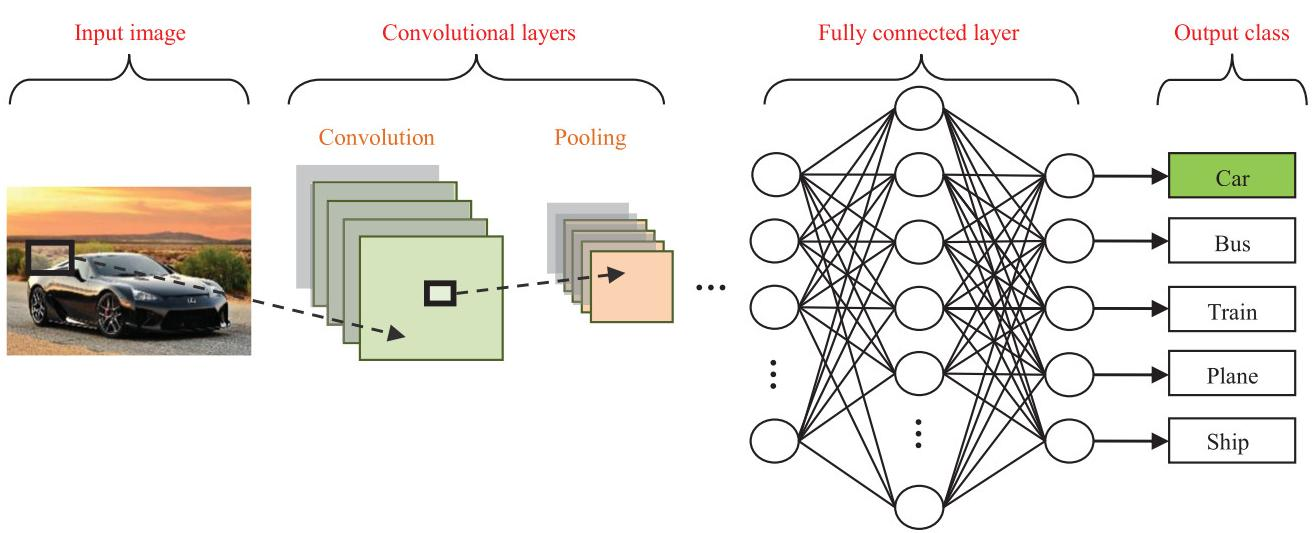
\includegraphics[width=0.95\textwidth]{img/cnn.jpg}
    \caption{Modelo visual da arquitetura de uma CNN \cite{Rawat_Wang_2017}.}
    \label{fig:cnn}
\end{figure}

\begin{figure}[htbp]
    \centering
    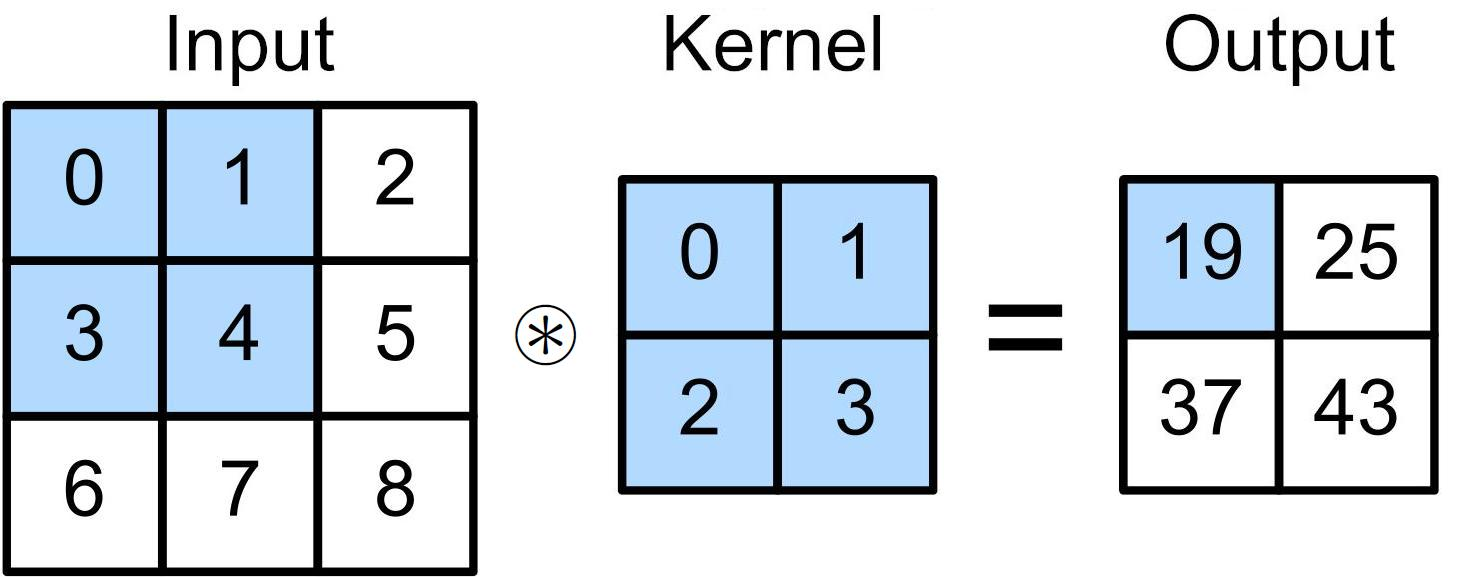
\includegraphics[width=0.7\textwidth]{img/conv.jpg}
    \caption{Exemplo de convolução ($\circledast$) numa entrada 2D de $3\times3\times1$ por um filtro (\textit{kernel}) $2\times2\times1$, com \textit{stride} de 1 (para altura e largura) e sem \textit{padding}. Operação de convolução para a posição $(0, 0) = 0 * 0 + 1 * 1 + 3 * 2 + 4 * 3 = 19$ \cite{Zhang_2021}.}
    \label{fig:conv}
\end{figure}

\begin{figure}[htbp]
    \centering
    \subfigure[]{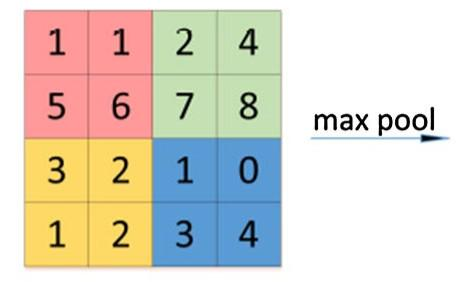
\includegraphics[height=0.2\textwidth]{img/pool1.jpg}}
    \subfigure[]{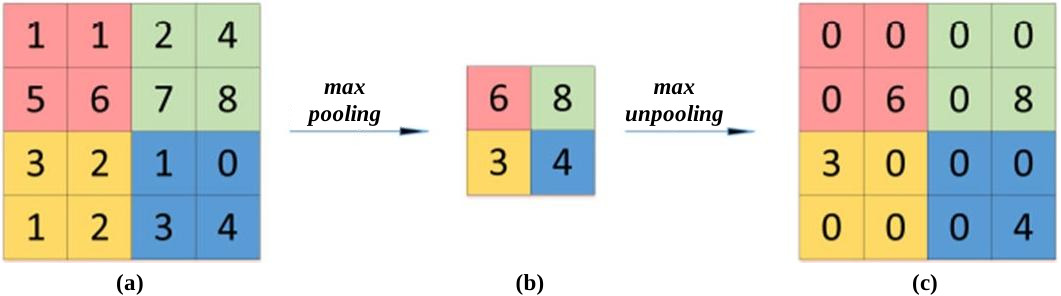
\includegraphics[height=0.2\textwidth]{img/pool2.jpg}}
    \subfigure[]{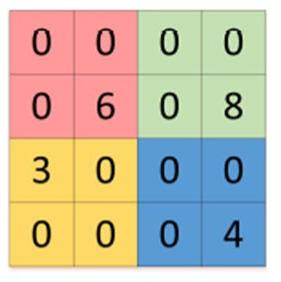
\includegraphics[height=0.2\textwidth]{img/pool3.jpg}}
    \caption{Exemplo de \textit{pooling} e \textit{unpooling}. (a) entrada 2D de $4\times4\times1$; (b) resultado da aplicação do \textit{max pooling} com janela de $2\times2$ e \textit{stride} de 2; (c) resultado da aplicação do \textit{unpooling} (\textit{max unpooling}) (a posição dos valores é guardada na operação de \textit{pooling}) \cite{Fang_2017}.}
    \label{fig:pooling}
\end{figure}

Algumas das arquiteturas de CNNs mais conhecidas incluem AlexNet, VGGNet e ResNet \cite{Minaee_2021}. Uma CNN consegue classificar uma imagem para uma das várias categorias que foi treinada ou reconhecer a presença de um objeto em qualquer parte da imagem analisada. Por outro lado, para a segmentação de imagens a informação espacial precisa ser preservada, por isso outros modelos de redes (e suas variações) são utilizadas \cite{Ponti_2017}.

Muitos modelos (algoritmos) de DL foram (e estão sendo) desenvolvidos para segmentação de imagens, e.g., redes totalmente convolucionais, U-net, Linknet, PSPNet. Nelas a saída terá o mesmo tamanho da entrada (ou pouco menor), contendo uma segmentação da imagem de entrada. Elas podem ser treinadas a partir do zero com os dados a serem segmentados, ou utilizar modelos pré-treinados (\textit{transfer learning}) com \textit{datasets} (como o ImageNet), além de serem utilizados variados \textit{backbones} como extratores de características \cite{Hao_2020, Minaee_2021}. Dentre as CNNs, a VGGNet e a ResNet são as mais utilizadas como \textit{backbones} \cite{Lateef_2019}.

As redes totalmente convolucionais (do inglês \textit{Fully Convolutional Netwoks} (FCNs)) (\autoref{fig:fcn}) são baseadas nas CNNs, onde a camada totalmente conectada é removida e sendo adicionado camadas de \textit{unpooling} e de \textit{transposed convolution} (convolução transposta).
O \textit{unpooling} (\autoref{fig:pooling}), ao contrário do \textit{pooling}, gera um mapa de características de maior resolução como saída. Outrossim a \textit{transposed convolution} (\autoref{fig:transposteConv}), as vezes chamada de \textit{deconvolution}, mesmo que a operação executada não é o oposto da convolução, também é aplicada de modo a aumentar a resolução do mapa de características \cite{Long_2015, Fang_2017}. 
\begin{figure}[htbp]
    \centering
    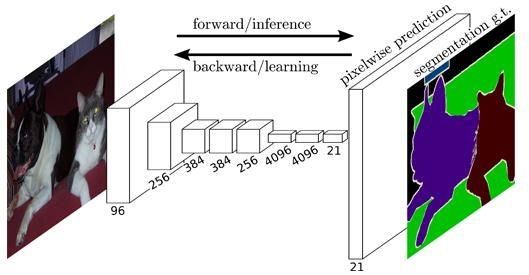
\includegraphics[width=0.6\textwidth]{img/fcn.jpg}
    \caption{Arquitetura simplificada de uma FCN \cite{Long_2015}.}
    \label{fig:fcn}
\end{figure}

\begin{figure}[htbp]
    \centering
    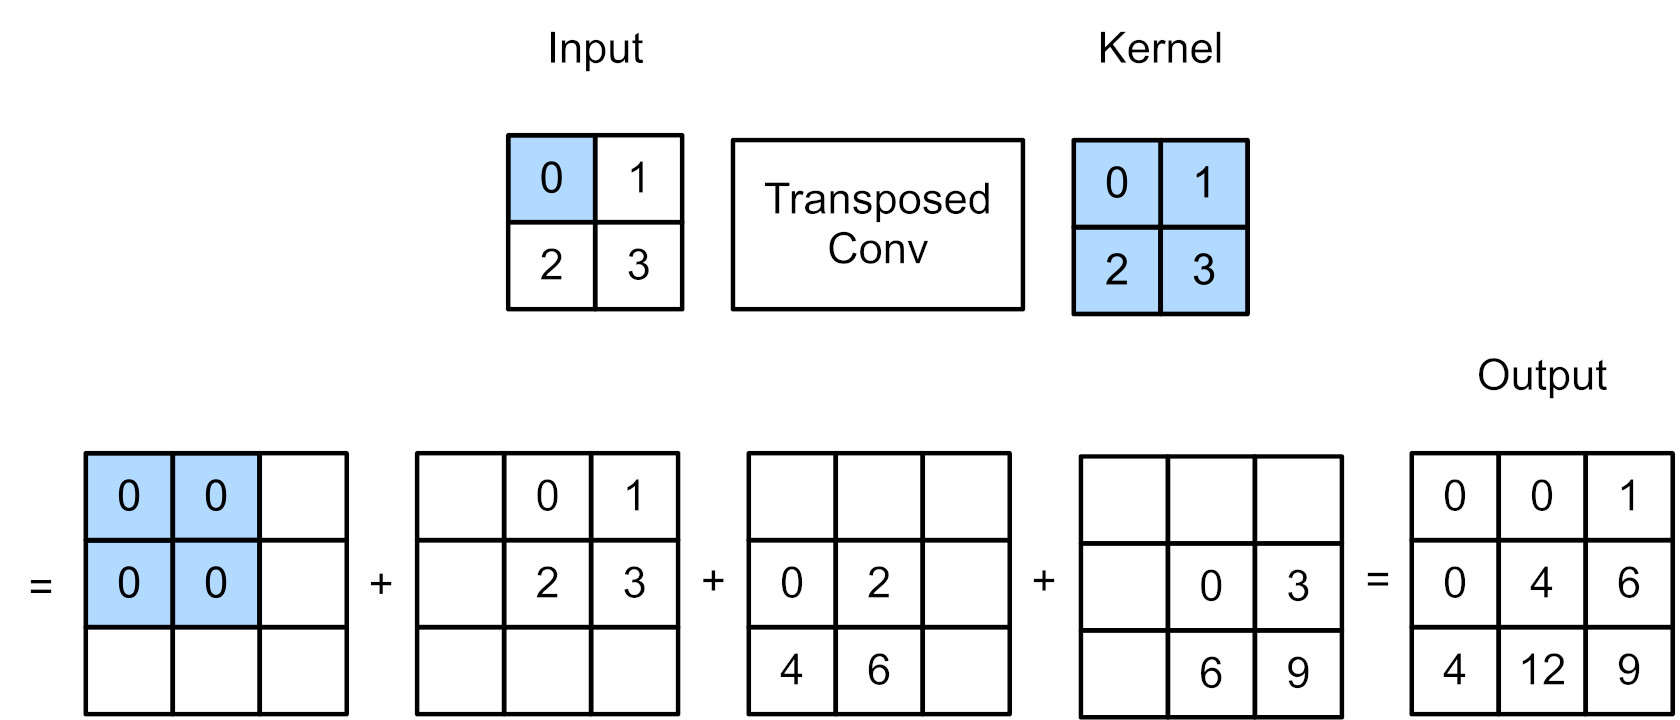
\includegraphics[width=0.7\textwidth]{img/trans_conv.jpg}
    \caption{Exemplo de convolução transposta numa entrada 2D de $2\times2\times1$ por um filtro (\textit{kernel}) $2\times2\times1$, com \textit{stride} de 1 (para altura e largura) e sem \textit{padding} \cite{Zhang_2021}.}
    \label{fig:transposteConv}
\end{figure}

A U-net (\autoref{fig:unet}), usada inicialmente para segmentar imagens médicas, foi baseada nas FCNs. Ela apresentada um formato em U (dando nome a rede), sendo simétrica: na primeira metade tem-se o \textit{encoder}, reduzindo os mapas de características e na outra metade o decoder expandindo eles até o tamanho de entrada original. A U-net tem \textit{skip connection} como as FCN, contudo aqui os mapas de características também são concatenado com seu simétrico na outra metade \cite{Ronneberge_2015, Hao_2020}

\begin{figure}[htbp]
    \centering
    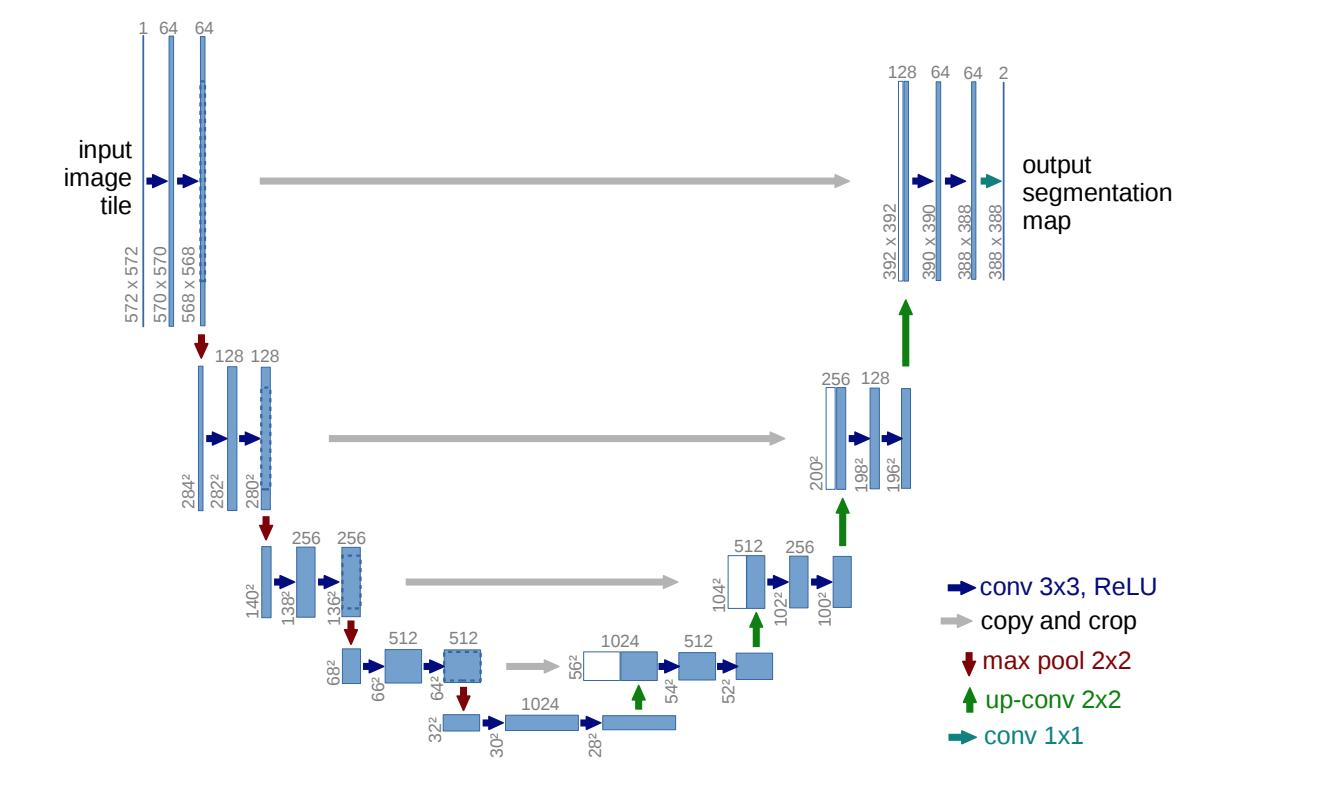
\includegraphics[width=0.85\textwidth]{img/unet.jpg}
    \caption{Arquitetura da U-net \cite{Ronneberge_2015}.}
    \label{fig:unet}
\end{figure}

A Linknet (\autoref{fig:linknet}) é similar a U-net, contudo utiliza  \textit{residual blocks} (blocos residuais) no \textit{encoder} e \textit{decoder}. Ela foi desenvolvida tendo como foco a segmentação semântica, com a arquitetura da ResNet de base. Os \textit{residual blocks} (\autoref{fig:residual_block}), também chamados de \textit{shortcut connections}, são úteis no problema de \textit{vanishing gradient} (dissipação do gradiente) em redes muito profundas, pois enviam o resultado para uma ou mais camadas a frente \cite{Chaurasia_2017, Ebrahimi_2021}.

\begin{figure}[htbp]
    \centering
    \subfigure[]{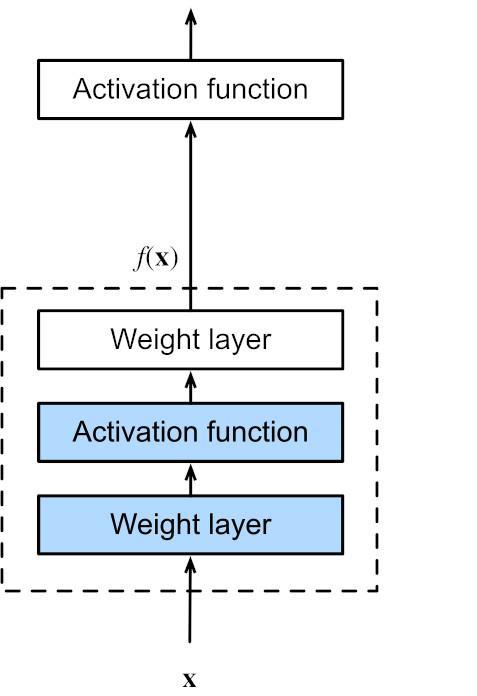
\includegraphics[height=0.45\textwidth]{img/residual_block1.jpg}}
    \subfigure[]{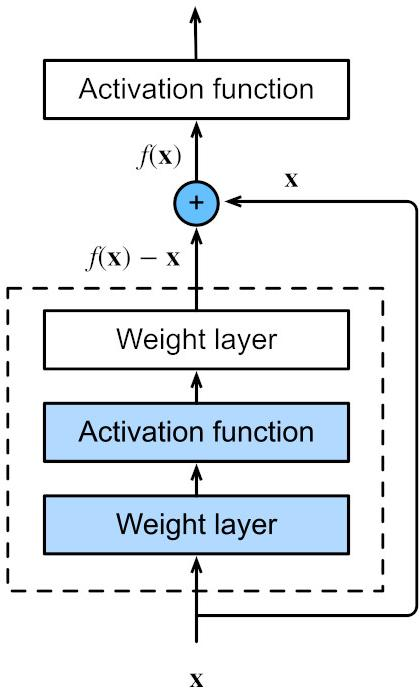
\includegraphics[height=0.45\textwidth]{img/residual_block2.jpg}}
    \caption{Exemplo de \textit{residual block}. (a) bloco regular; (b) bloco residual, onde a linha sólida leva a entrada $\textbf{x}$ até operador de adição, propagando mais rápido pela rede \cite{Zhang_2021}.}
    \label{fig:residual_block}
\end{figure}

\begin{figure}[htbp]
    \centering
    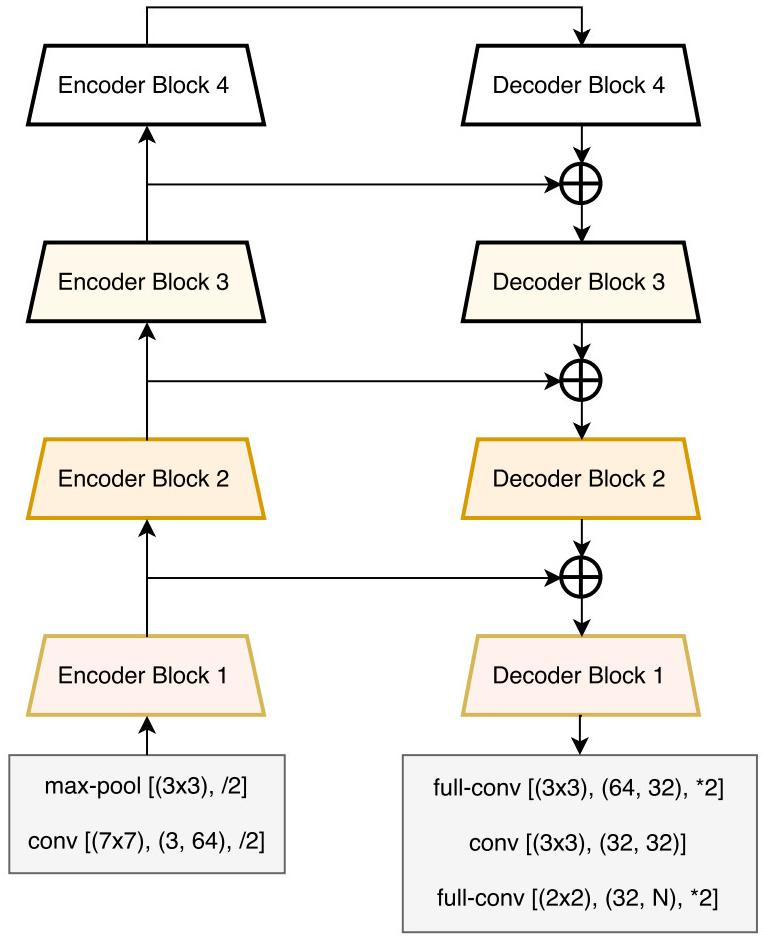
\includegraphics[width=0.55\textwidth]{img/linknet.jpg}
    \caption{Arquitetura da Linknet \cite{Chaurasia_2017}.}
    \label{fig:linknet}
\end{figure}

%\textRed{Segnet}

A \textit{Pyramid Scene Parsing Network} (PSPNet) (\autoref{fig:pspnet}) utiliza o módulo \textit{pyramid parsing}, que explora informações de contexto global através de diferentes regiões baseadas em agregação de contexto. As informações locais e globais são agrupadas para fazer uma predição final de maior confiança. Por base a PSPNet utiliza uma ResNet pré-treinada utilizando \textit{dilated convolution} (convoluções dilatadas) como extratores de características. As \textit{dilated convolution} (\autoref{fig:dilated_conv}) são um tipo de convolução que dilata o filtro ao inserir espaços entre os valores do mesmo. Os espaços são definidos pelo parâmetro $l$, a taxa de dilatação, com $l = 1$ é a convolução tradicional, já $l > 1$ são convoluções dilatadas \cite{Zhao_2017, Minaee_2021}.

\begin{figure}[htb]
    \centering
    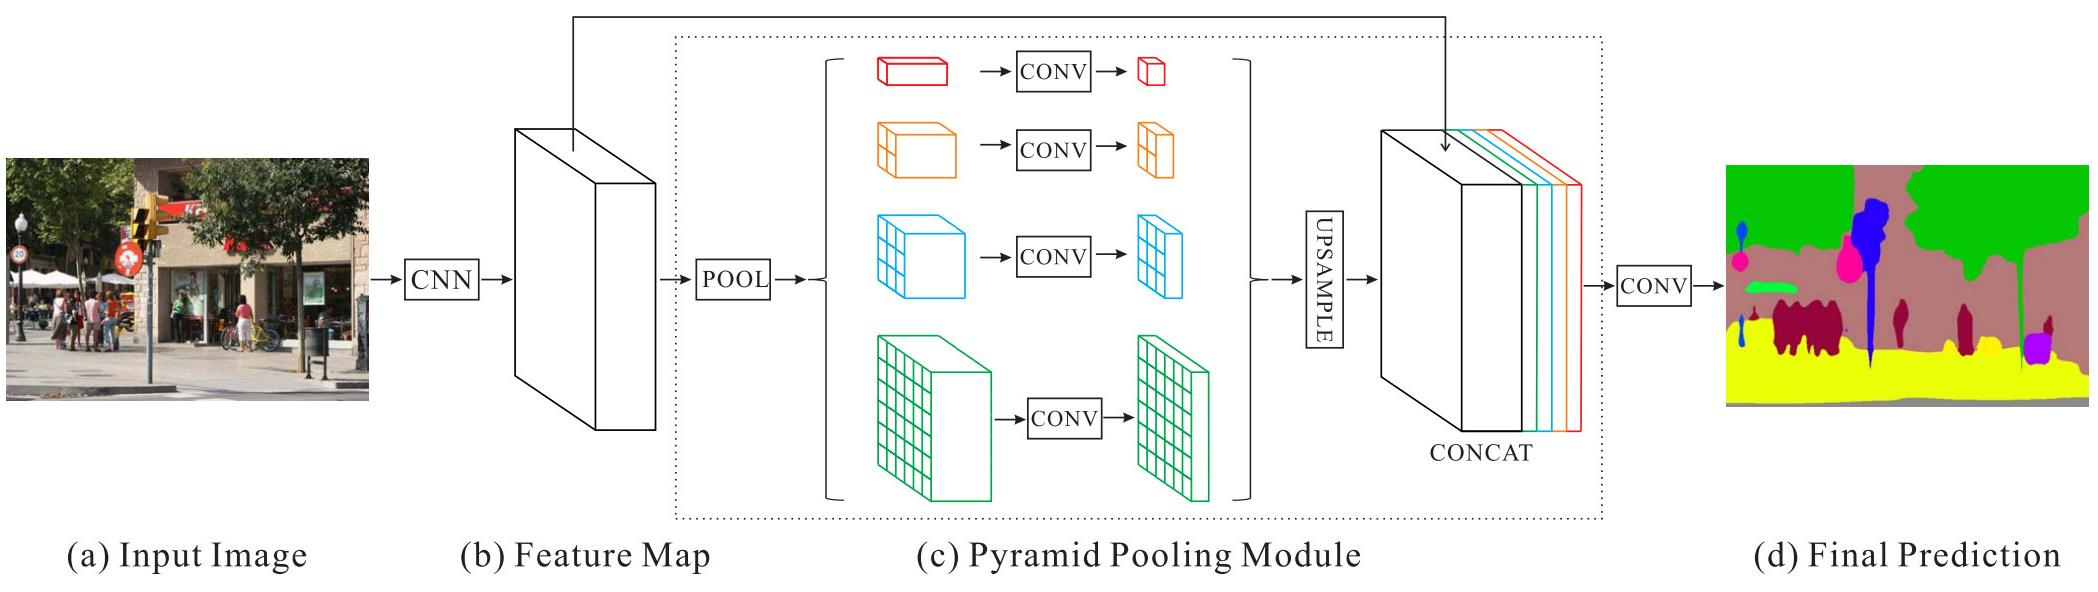
\includegraphics[width=0.99\textwidth]{img/pspnet.jpg}
    \caption{Arquitetura da PSPNet \cite{Zhao_2017}.}
    \label{fig:pspnet}
\end{figure}

\begin{figure}[htb]
    \centering
    \subfigure[]{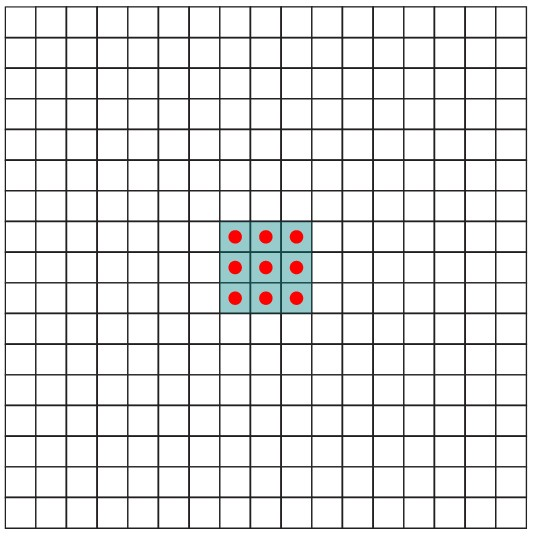
\includegraphics[height=0.25\textwidth]{img/dilated_conv1.jpg}}
    \subfigure[]{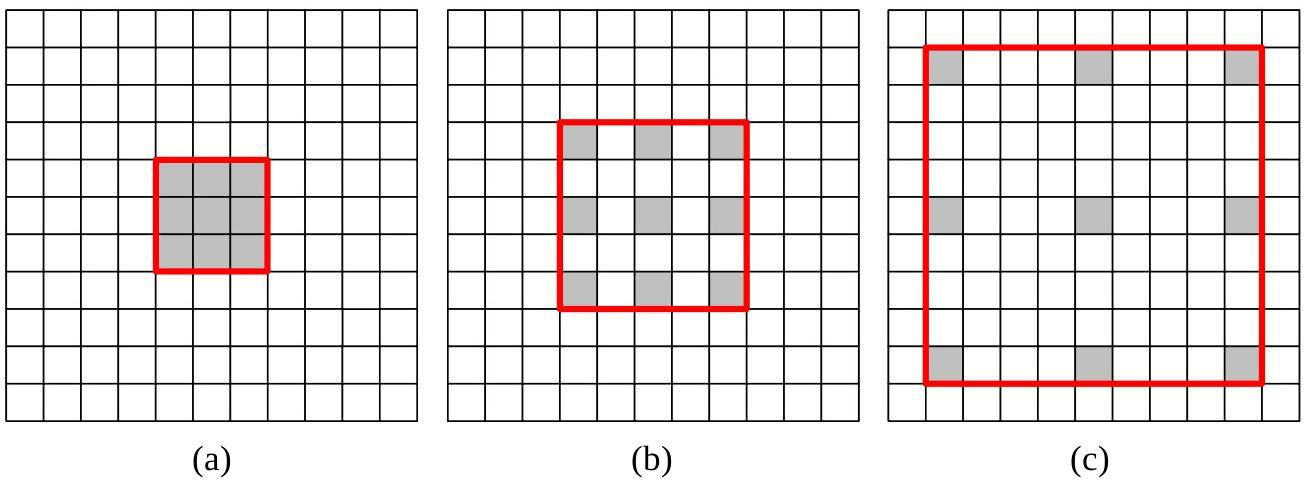
\includegraphics[height=0.25\textwidth]{img/dilated_conv2.jpg}}
    \subfigure[]{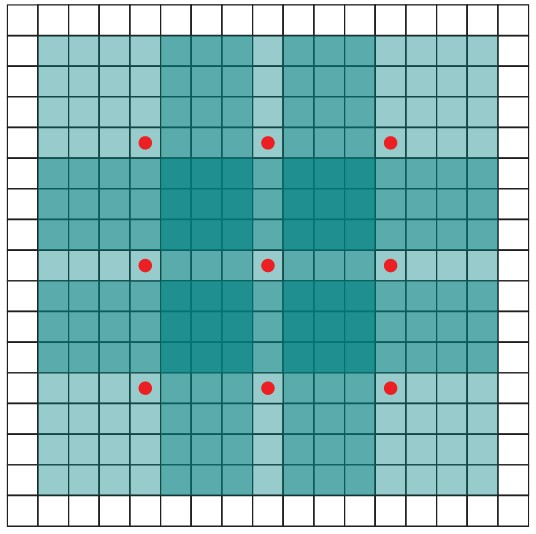
\includegraphics[height=0.25\textwidth]{img/dilated_conv3.jpg}}
    \caption{Exemplo de \textit{dilated convolution} com 3 valores de dilatação ($l$).; (a) $l = 1$; (b) $l = 2$; (c) $l = 4$ \cite{Minaee_2021}.}
    \label{fig:dilated_conv}
\end{figure}

% \dotsBlue

% \clearpage % force all image be placed

\subsection{Trabalhos relacionados}

Nesta seção serão discutidos alguns trabalhos (recentes) relacionados que servirão de base para o desenvolvimento de novas metodologias para segmentação de imagens de VANTs associadas a AP e a detecção de linhas de plantio.

\citeonline{Souza_2017} desenvolveram um método para detectar linhas de plantio em imagens de VANTs de plantações de cana-de-açúcar (GSD de aproximadamente 0.10 m) e suas falhas. Para a análise das imagens e para a execução do processo de análise de imagem baseada em objeto (OBIA), foi utilizado o \textit{software} comercial \textit{eCognition Developer}\footnote{https://geospatial.trimble.com/products-and-solutions/ecognition} 8 (\textit{Trimble GeoSpatial}). A OBIA primeiramente identifica unidades espacialmente e espectralmente homogêneas, chamadas de ``objetos'', criados pelo agrupamento de pixels adjacentes e, em seguida, os utiliza como elementos básicos para análise. Para identificar as linhas de plantio foi utilizado o NDVI (as imagens utilizadas têm as bandas RGB e a NIR). Também foi utilizado o \textit{software} comercial \textit{Arcgis}\footnote{https://www.esri.com/en-us/arcgis/products/arcgis-pro/overview} (Esri) para extrair automaticamente falhas nas linhas (através do ``\textit{ModelBuilder}''). O método foi avaliado comparando 54 falhas estimadas pelo método e as observadas (medição por fita métrica). Apesar dos resultados estimados serem próximo dos observados, o método apresenta limitações em relação aos \textit{softwares} comerciais utilizados e aos poucos testes que foram realizados.

\citeonline{Garcia_2017} desenvolveram um método para identificar linhas retas e curvas em plantações de milho. As imagens são de baixíssima altitude (2 m, câmera acoplada no maquinário agrícola). Para a segmentação foi utilizado o índice de vegetação ExG (para facilitar a diferenciação de plantas e ervas daninhas do solo), em seguida é aplicado o método de Otsu com dois limiares (dividindo a imagem em 3 classes: milho, erva daninha e solo) e depois operações morfológicas são aplicadas. Após a segmentação, a TH foi utilizada para identificar 4 pontos - começos de linhas de plantio na imagem (necessário para o veículo autônomo se guiar).


\textRed{Esse 4 pontos são as linhas de plantio esperada para estar presentes nas imagens e são identificadas até certa distância a frente, assim podendo ser tratadas como linhas retas. Imagens com menos de 4 começos de linhas são rejeitadas} \dotsBlue

\linePage

\citeonline{Souza_2018} \dotsBlue
café e cana

HT
curva
linhas e escolhas das linhas
algoritmo

\linePage

\citeonline{Soares_2018} comentam que a TH é uma boa escolha inicial para detectar linhas de plantio, justificando vários trabalhos anteriores utilizarem esse método. Contudo a TH necessita que o formato do objeto a ser detectado seja conhecido antecipadamente, o que limita sua utilização para detectar as linhas de plantio. Para mitigar essa limitação, no trabalho utilizam a TH com o esquema janelamento (\textit{tiling scheme}), onde as linhas de plantio se aproximam de linhas retas. No método desenvolvido a TH foi aplicada com o janelamento com variados tamanhos de janela e porcentagem de sobreposição. O método foi avaliado em 8 imagens de VANTs de plantações de café e suas marcações feitas por um especialista. Os melhores resultados foram com janela de 200 pixels e sobreposição de 48 \%. A sobreposição ajuda evitar descontinuidades nas linhas detectadas.

\linePage

\citeonline{Rozo_2019} \dotsBlue
Gis - plugin
semente, direção da imagem-mosaico
linhas retas
cana
\linePage

\citeonline{Bah_2020} \dotsBlue
dl
ht
cnn
cana

\linePage

Em \citeonline{Silva_2020} foram desenvolvidas duas abordagens para detecção de linhas de plantio de cana-de-açúcar, a primeira utilizando Algoritmo Genético (AG) resultando em \citeonline{Silva_Escarpinati_Backes_2021} e a segunda utilizando redes neurais artificiais. Para comparar os resultados, foram utilizados 4 \textit{datasets} (com plantas de variadas idades) e suas respectivas linhas de plantio, marcadas por um especialista. O AG foi utilizado para encontrar uma máscara (filtro convolucional que combina as bandas RGB da imagem para uma em escala de cinza), que maximize o Coeficiente de Dice (CD). Em sequência o método Otsu foi utilizado para binarizar as imagens e por fim, a TR foi utilizada para refinar a detecção das linhas de plantio. Como resultado, a detecção das linhas ficou próximas da marcação do especialista, lidando melhor com linhas retas e não muito bem com linhas curvas (gerando um efeito de serrilhamento indesejado). Na abordagem com redes neurais, a LinkNet apresentou melhor resultado que na abordagem anterior. A TR também foi aplicada nessa abordagem, contudo piorando o desempenho em muitos casos.

\linePage

\citeonline{Oliveira_2020} desenvolveu uma abordagem similar a \citeonline{Silva_2020}, para a detecção das linhas de plantio de cana-de-açúcar. Nela, o mosaico é dividido em pequenas imagens, que são convertidas para escala de cinza e feita redução dos níveis de cinza (de 256 para 32) pela Transformada Discreta de Wavelet. Na sequência, o AG é utilizado para encontrar 4 limiares, o maior é usado para segmentar a imagem, que segue para operações morfológicas de fechamento, erosão e esqueletização. Por fim a Transformada de Hough Probabilística Progressiva é utilizada para otimizar a detecção das linhas de plantio e suas falhas. O trabalho apresenta um bom resultado, mas foi aplicado apenas em uma pequena seção do mosaico, sem um padrão ouro para teste e considera as linhas de plantio como linhas retas.

\linePage

\citeonline{Pereira_Junior_2020} \dotsBlue
algoritmos tradicionais
cana
\linePage

\citeonline{Barbosa_Junior_2021} fez uma análise exploratória do uso de imagens de VANTs na detecção das falhas nas plantações de cana-de-açúcar, variando o GSD (3.5 cm, 6 cm e 8.2 cm), a altura da planta (0.5 m, 0.9 m, 1.2 m e 1.7 m), e o comprimento das falhas (0.5 m, 1.0 m, 1.5 m, 2.0 e 2.5 m). Na identificação das falhas foi utilizado o \textit{software} comercial \textit{Inforow} \cite{Inforow_2021}. Como esperado, os melhores resultados foram com GSD pequeno (3.5 cm ou próximo) e plantas com menor altura (e.g., 0.5 m). A altura das plantas foi apontada como um dos fatores mais importantes, seguido pelo GSD, para detecção das falhas nas plantações de cana-de-açúcar. Não foi possível detectar pequenas falhas $(\le 1$ m$)$ quando a planta já tinha certa altura $(\ge 1$ m$)$ através do \textit{software}. É importante notar que mesmo o \textit{software} comercial não obteve bons resultados em certos cenários.

\linePage

\textRed{parágrafo comentando os principais trabalhos de modo bem resumido}

Na literatura, o trabalho de \citeonline{Silva_2020} contribuiu significativamente para detecção das linhas de plantio em plantações de cana-de-açúcar, contudo não obteve bons resultados com linhas curvas (gerando um efeito serrilhamento indesejado). Por outro lado a abordagem com redes neurais teve melhor resultado, mas ainda pode ser melhor explorada. \citeonline{Oliveira_2020} apresenta uma abordagem similar, mas que não foi muito bem testada.  \dotsBlue.


\section{Metodologia de pesquisa}
% => Descreva de forma mais detalhada sua proposta de trabalho, detalhando as estratégias que pretende utilizar para atingir os objetivos propostos. Descreva o método de pesquisa que deverá ser utilizado para validar a sua hipótese incluindo as medidas de avaliação, conjunto de parâmetros, bases de dados e os trabalhos com os quais a sua proposta será comparada.

A metodologia deste projeto é composta por 5 etapas. A primeira etapa é a aquisição das imagens/\textit{datasets} coletadas por VANTs utilizando uma câmera RGB em plantações de cana-de-açúcar. A segunda etapa é o pré-processamento dessas imagens, buscando realçar as linhas de plantio e corrigir pequenas imperfeições.

A terceira etapa é o processamento principal, ou seja, a segmentação das imagens. Nela serão testados e propostos métodos para melhorar a segmentação dessas imagens. Na quarta etapa será feito o pós-processamento para otimizar a segmentação e refinar as linhas detectadas pela etapa anterior, além de tratar linhas incompletas e linhas curvas. Por fim, será feita a avaliação dos resultados da detecção das linhas de plantio.

\subsection{Aquisição das imagens}

As imagens para os experimentos são de VANTs em culturas, inicialmente, de cana-de-açúcar e de \textit{datasets} disponíveis. Dentre os \textit{datasets}, poucos utilizam imagens de VANTs. Em \citeonline{Silva_2020} 4 mosaicos (\autoref{fig:mosaicos1}) de plantações de cana-de-açúcar e suas respectivas linhas de plantio (\autoref{fig:linhas}), marcadas por um especialista, foram utilizadas. As imagens foram capturadas por um VANT de mapeamento, modelo \textit{eBee SenseFly}, com uma câmera \textit{SenseFly S.O.D.A.} de uma polegada, tendo $5472\times3648$ pixels de resolução e lente RGB F/2.8-11, 10.6 mm. Cada pixel na imagem representa aproximadamente 5 cm (GSD de 0,053 m). Esses mosaicos têm canas-de-açúcar em variados estágios (idades). As marcação do especialista foram feitas onde existe a linha de plantio e também onde deveria existir, ou seja, locais de falhas no plantio também foram marcados como linha de plantio.

\begin{figure}[htbp]
    \centering
    \subfigure[]{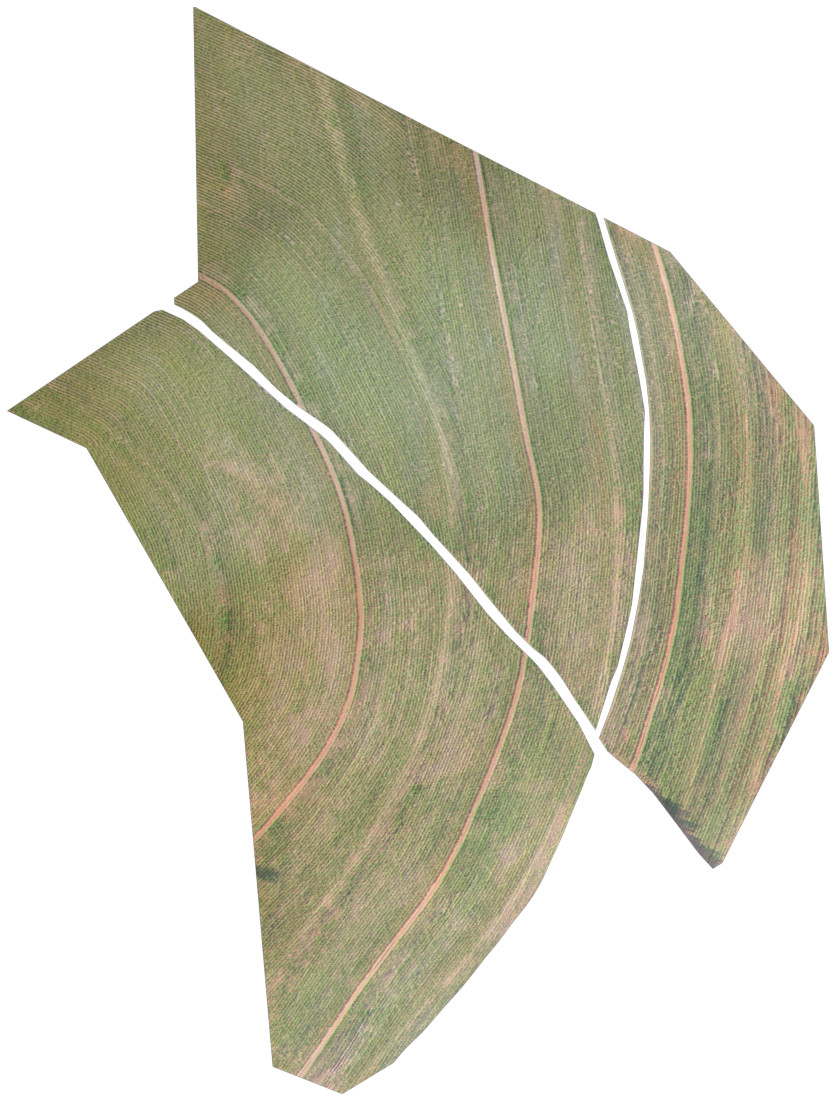
\includegraphics[width=0.12\textwidth]{img/a2.jpg}} 
    \subfigure[]{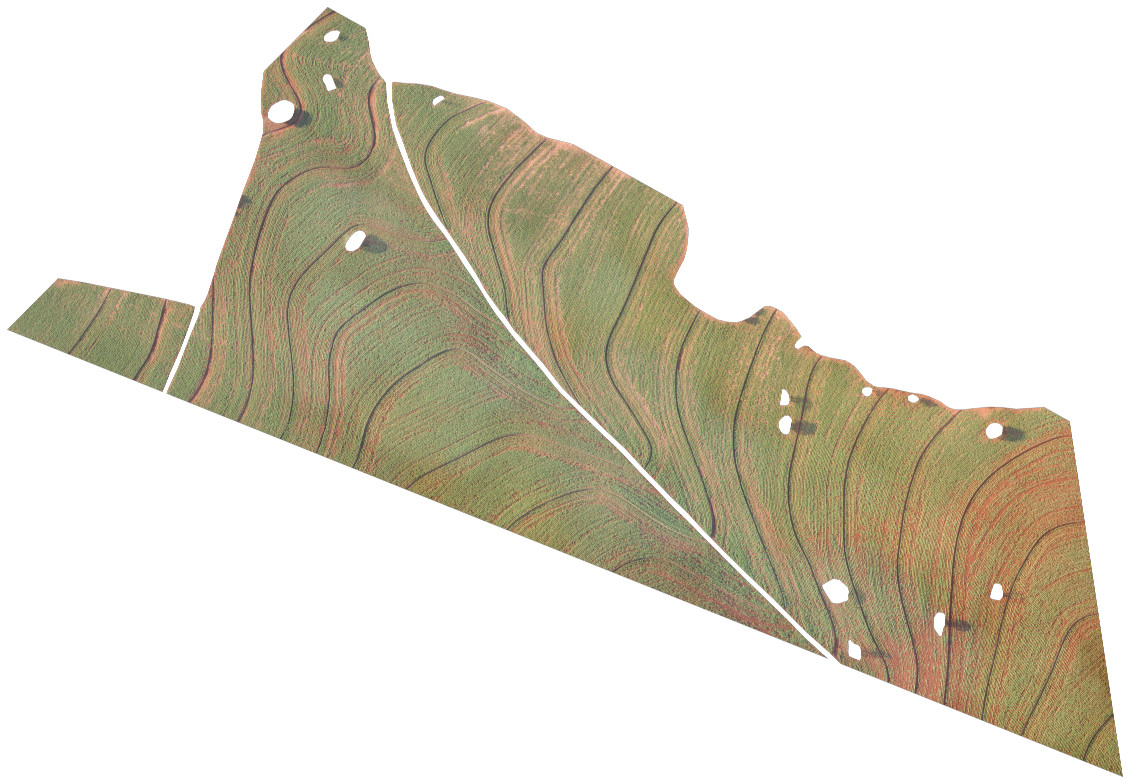
\includegraphics[width=0.31\textwidth]{img/b2.jpg}} 
    \subfigure[]{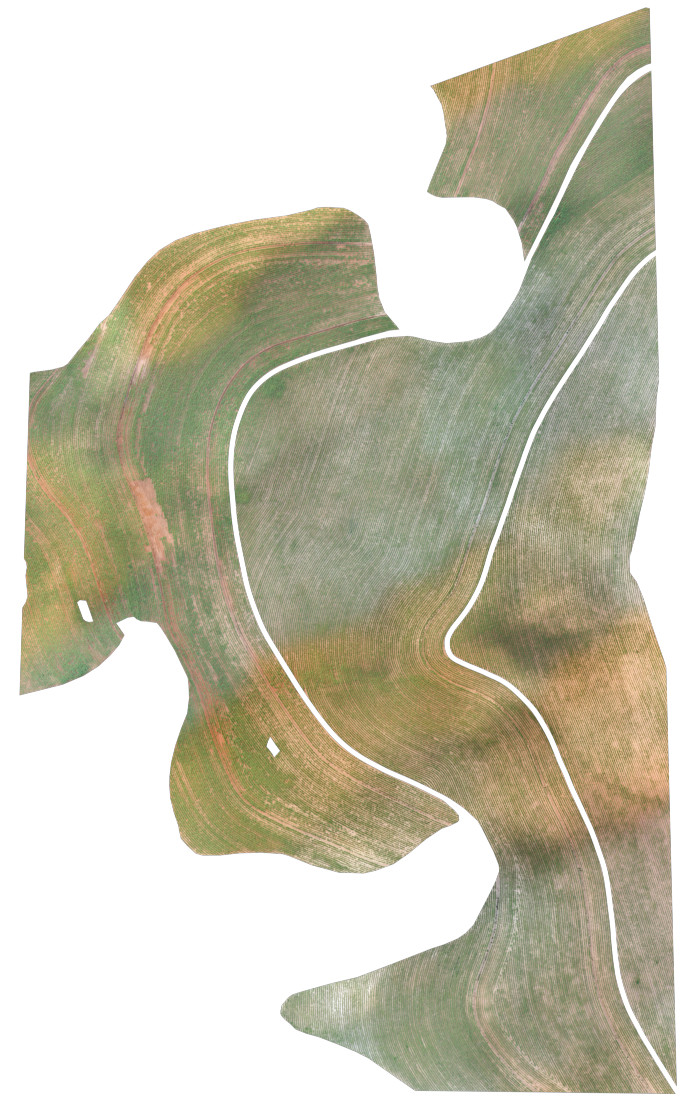
\includegraphics[width=0.14\textwidth]{img/c2.jpg}}
    \subfigure[]{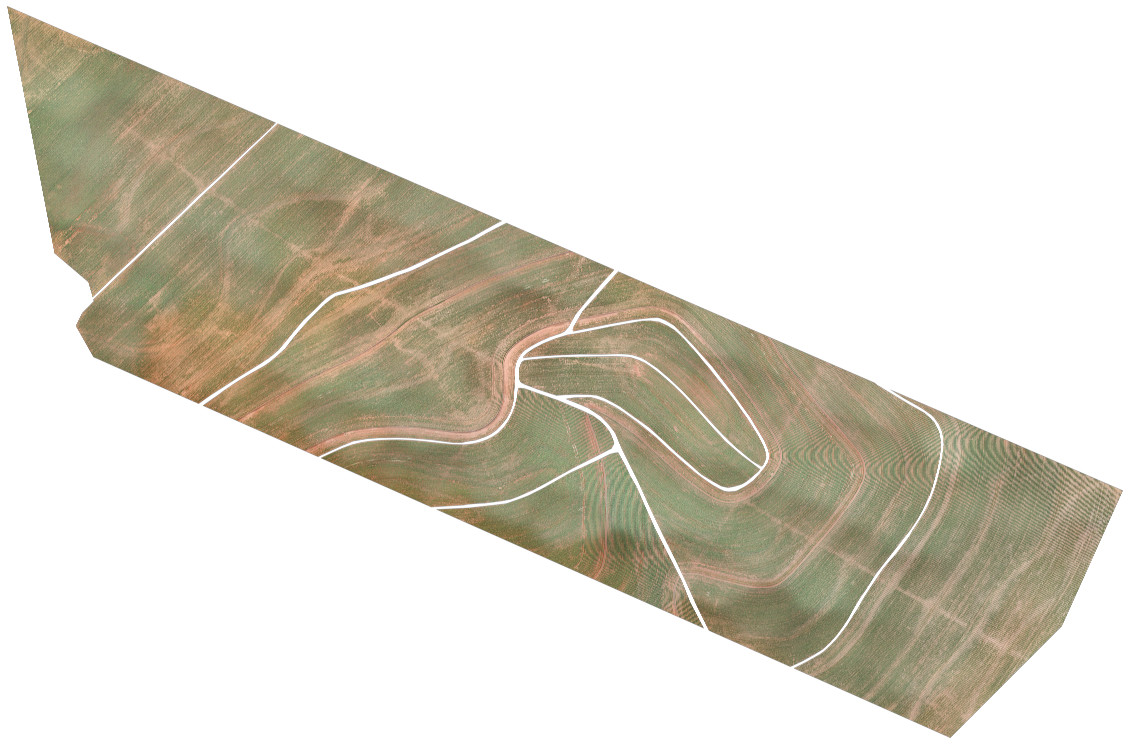
\includegraphics[width=0.40\textwidth]{img/d2.jpg}}
    \caption{Mosaicos e seus respectivos tamanhos: (a) 11180 $\times$ 8449; (b) 16677 $\times$ 24181; (c) 17497 $\times$ 10771; (d) 19833 $\times$ 30255.}
    \label{fig:mosaicos1}
\end{figure}

\begin{figure}[htbp]
    \centering
    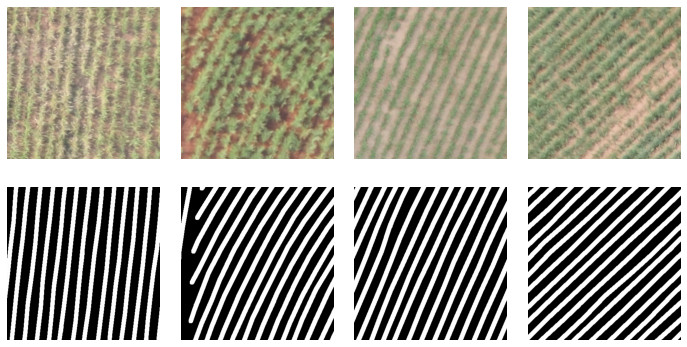
\includegraphics[width=0.8\textwidth]{img/linhas2.jpg}
    \caption{Exemplos de marcações feitas pelo especialista nos 4 mosaicos em \citeonline{Silva_2020}.}
    \label{fig:linhas}
\end{figure}

Em \citeonline{Pereira_Junior_2020}, utilizaram 1 mosaico \cite{CropRowsDataset2019} (\autoref{fig:mosaicos2}) capturado com uma câmera RGB \textit{Canon G9X} e VANT \textit{Horus Aeronaves}, resultando em um GSD aproximado de 5 cm. O mosaico foi marcado por um especialista; as linha de plantio em verde, o fundo/solo em vermelho, já fora do mosaico todos pixels foram definidos como pretos.

\begin{figure}[htbp]
    \centering
    \subfigure[]{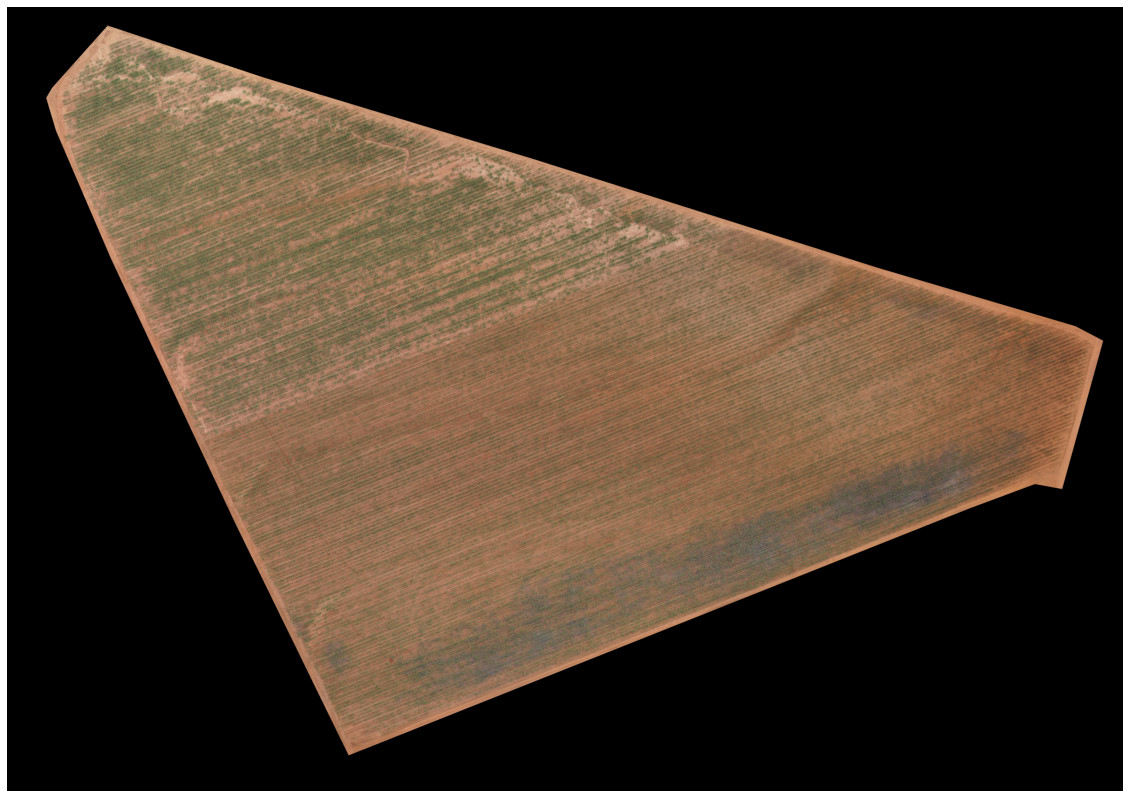
\includegraphics[width=0.49\textwidth]{img/sugarcane1-s2.jpg}} 
    \subfigure[]{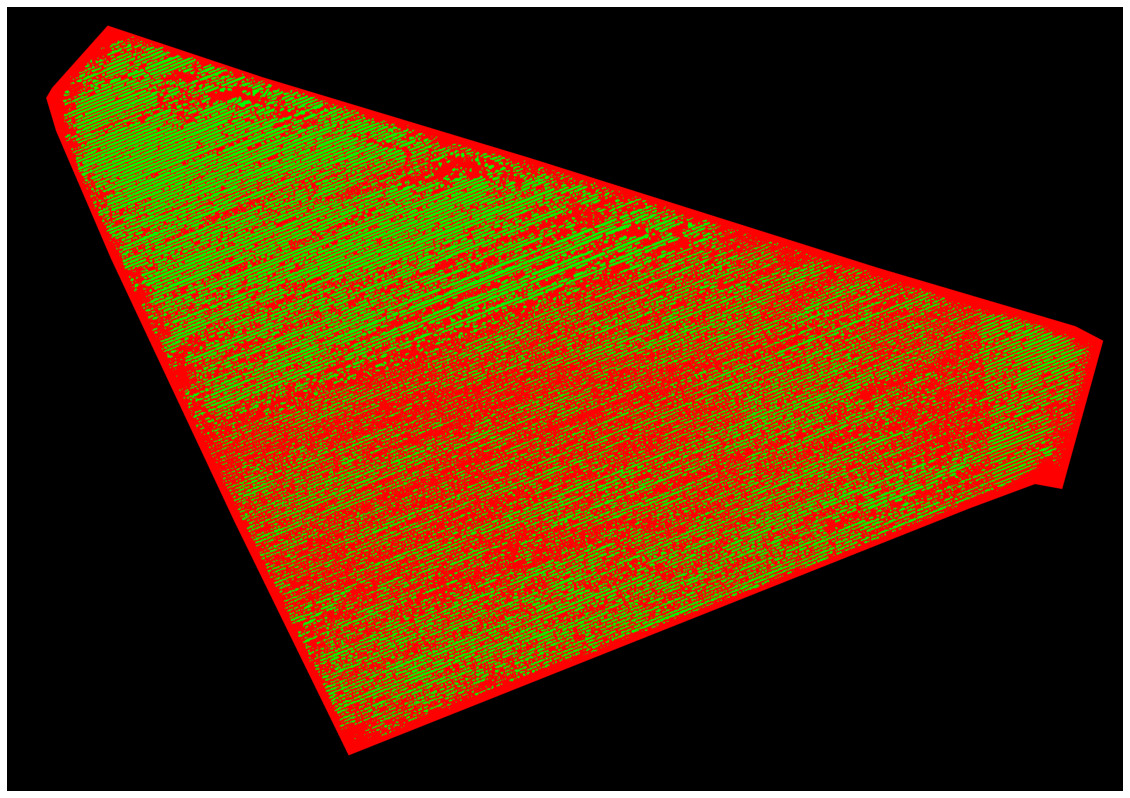
\includegraphics[width=0.49\textwidth]{img/sugarcane1-GT-s2.jpg}} 
    \caption{Mosaico \citeonline{CropRowsDataset2019}: (a) mosaico de tamanho (incluindo bordas pretas) 6595 $\times$ 9391; (b) marcação do especialista (de mesmo tamanho).}
    \label{fig:mosaicos2}
\end{figure}

Além dos dois \textit{datasets} disponíveis, pretende-se capturar novos mosaicos, dependendo da demanda dos experimentos, de culturas de cana-de-açúcar e outras, através dos VANTs. Depois também será feita neles a marcação por um especialista, destacando as linhas de plantio do solo/fundo.

\subsection{Pré-processamento}

No pré-processamento serão feitos ajustes nas imagens de modo a facilitar ou melhorar os resultados da segmentação. Dentre eles a correção de brilho e contraste, quando forem necessário, além da remoção de ruídos que podem estar presentes nas imagens. Após converter as imagens para níveis de cinza, as operações morfológicas podem ser úteis.

A dilatação pode ser utilizada para juntar plantas isoladas de suas respectivas linhas de plantio devido a pequenas falhas, assim expandir extremidades e conectar elas com a linha de plantio. Por outro lado, a erosão, pode ser utilizada para separar estreitos e compridos filamentos onde plantas podem estar ligadas com outras linhas de plantio ou com uma errada.

\subsection{Segmentação}

A próxima etapa é a segmentação, que as vezes é chamada de processamento principal, devido a sua importância e complexidade. Inicialmente é importante conhecer as imagens que serão segmentadas e quais métodos de segmentação serão utilizados. Para este projeto serão utilizadas imagens de VANTs com as bandas RGB. De modo a ficar mais barato as suas capturas do que de imagens com banda infravermelho e/ou infravermelho próximo, pois essas precisam de uma câmera específica que consiga capturar tais bandas, contudo alguns informações úteis poderiam ser obtidas dessas bandas e IV (como o NDVI).

Como as imagens são de plantações de cana-de-açúcar (e de outras culturas, dependendo do desenvolvimento do projeto) é certo encontrar nelas fileiras da cultura e variadas partes de solo exposto. As culturas de cana-de-açúcar geralmente são classificadas em 4 fases de desenvolvimento (brotação e estabelecimento, perfilamento, crescimento de colmos e maturação), como pode ser visualizado na \autoref{fig:cana_estagios} \cite{Lu_Zhou_2019}.

\begin{figure}[htbp]
    \centering
    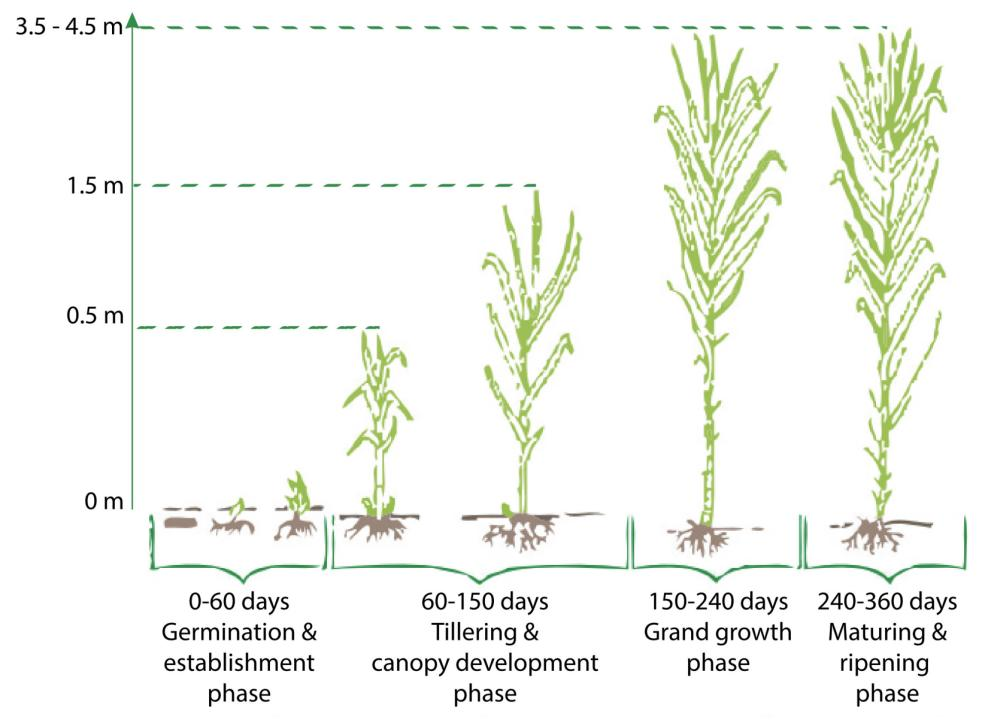
\includegraphics[width=0.95\textwidth]{img/cana_estagios.jpg}
    \caption{Fases de desenvolvimento da cana-de-açúcar: 0-60 dias, fase de brotação e estabelecimento; 60-150 dias, fase de perfilamento; 150-240, fase de crescimento dos colmos; 240-360 dias, fase de maturação) \cite{Molijn_2019}.}
    \label{fig:cana_estagios}
\end{figure}

Dentre as fases de desenvolvimento e seus respectivos dias, \citeonline{Souza_2017} recomenda que as imagens sejam capturadas entre 60-90 dias após o plantio (ou corte/colheita), quando a cana-de-açúcar já cresceu o suficiente para preencher a linha de plantio, mas sem cobrir os espaços entre as linhas. Entretanto esse período pode variar dependendo da variedade de cana-de-açúcar plantada, da quantidade plantas/socas na linha, da quantidade de chuva entre outros fatores. Assim, também é recomendado uma análise visual da plantação para confirmação do melhor momento para capturar as imagens.

Considerando que as imagens foram capturas dentre os períodos recomendados, é esperado ter uma boa visibilidade da linhas de plantio e das partes de solo exposto. Deste modo, dois cenários são mais esperados: com cana-planta e cana-soca, como na \autoref{fig:cana_planta_soca}. No estágio de cana-soca, o solo está coberto com folhas secas do último corte/colheita, dando aspecto amarelado, dificultando a análise computação, já no estágio de cana-planta o solo está mais visível.

\begin{figure}[htbp]
    \centering
    \subfigure[]{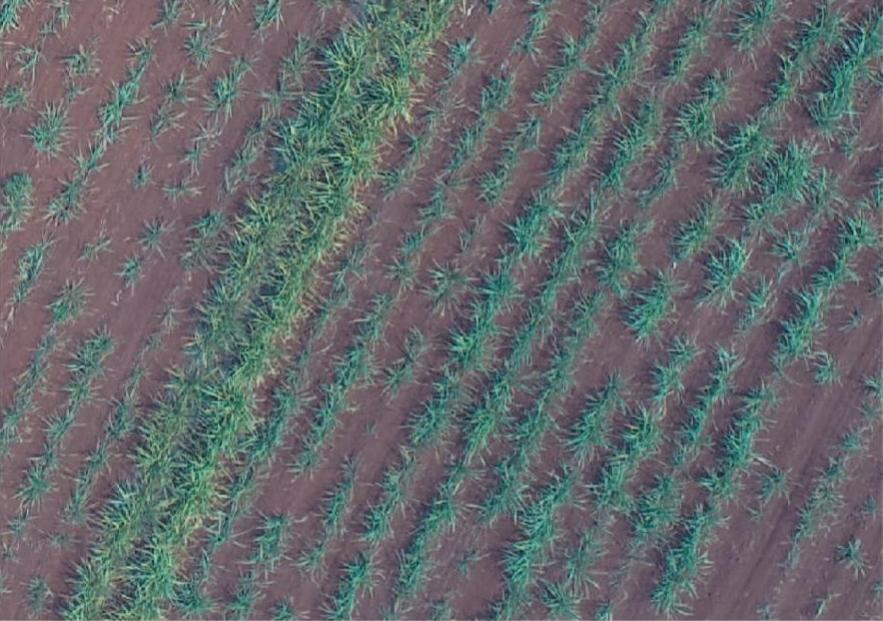
\includegraphics[width=0.49\textwidth]{img/cana_planta.jpg}} 
    \subfigure[]{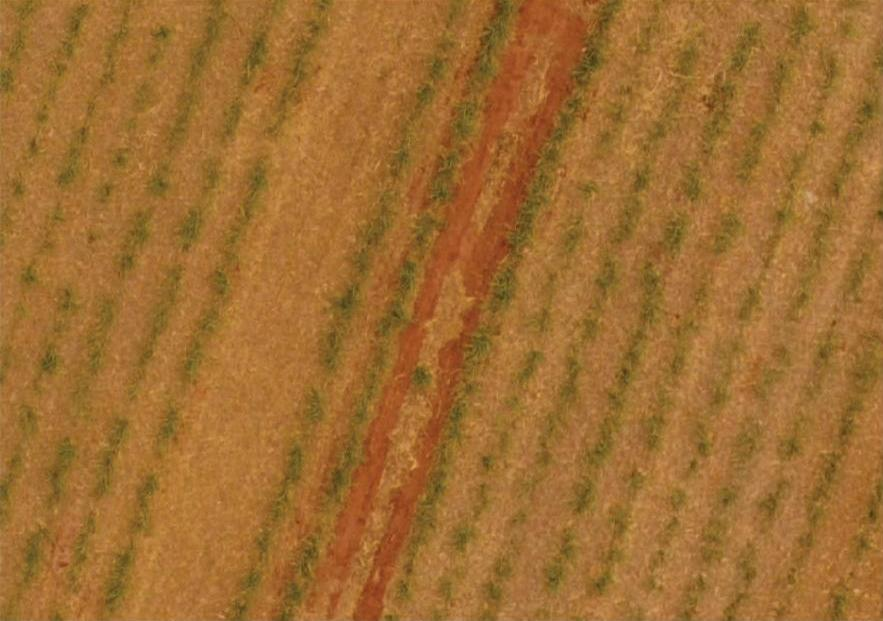
\includegraphics[width=0.49\textwidth]{img/cana_soca.jpg}} 
    \caption{Cana-de-açúcar: (a) estágio de cana-planta (após o plantio e o nascimento, mas antes do primeiro corte); (b) estágio de cana-soca (após o corte) \cite{Silva_2020}.}
    \label{fig:cana_planta_soca}
\end{figure}

Sobre os métodos de segmentação, neste projeto, inicialmente, foi escolhido as redes neurais para segmentar as imagens. Elas têm melhor resultado na segmentação, em comparação com os algoritmos tradicionais (e outros métodos como AG), por utilizar não apenas o tom avermelhado do solo e esverdado da plantas, mas outras características que elas conseguem extrair das imagens \cite{Silva_2020}. Dentre essas características, podem ser contornos, formatos de linhas e outros tipos de formatos específicos. 

As redes para segmentação (algumas apresentadas na \autoref{sec:dl}) serão treinadas para segmentar as linhas de plantio utilizando algumas abordagens. Elas serão treinadas com as imagens (RGB) das plantações, índices de vegetação, ou a combinação de ambos. Dentre os IVs para imagens RGB, alguns são mais utilizados, como o ExG, contudo vários outros podem ser utilizados, como pode ser visualizado na \autoref{tab:iv}. A utilização dos IVs é motivada pela hipótese de que as redes irão apreender mais características visuais das plantas e do solo do que apenas com a imagem RGB, sendo assim capaz de diferencia-los com maior precisão.

\begin{table}[htb]
    \centering
    \caption{Índices de Vegetação \cite{Lu_Zhou_2019}}
    \label{tab:iv}
    \begin{tabular}{@{}lll@{}}
        \toprule
        Índice & \multicolumn{1}{c}{Nome} & \multicolumn{1}{c}{Equação} \\ \midrule

        \multirow{2}{*}{VARI} & \multirow{2}{*}{\textit{Visible Atmospherically Resistant Index}} & \multirow{2}{*}{$\displaystyle \text{VARI} = \frac{g - r}{g + r - b} $} \\
        & & \\ \midrule

        \multirow{2}{*}{ExG} & \multirow{2}{*}{\textit{Excess Green Index}} & \multirow{2}{*}{$\displaystyle \text{ExG} = 2 * g - r - b$} \\
        & & \\ \midrule

        \multirow{2}{*}{ExR} & \multirow{2}{*}{\textit{Excess Red Vegetation Index}} & \multirow{2}{*}{$\displaystyle \text{ExR} = \frac{1,4 * R - G}{G + R + B} $ } \\
        & & \\ \midrule

        \multirow{2}{*}{ExB} & \multirow{2}{*}{\textit{Excess Blue Vegetation Index}} & \multirow{2}{*}{$\displaystyle \text{ExB} = \frac{1,4 * B - G}{G + R + B}$} \\
        & & \\ \midrule

        \multirow{2}{*}{ExGR} & \multirow{2}{*}{\textit{Excess Green minus Excess Red}} & \multirow{2}{*}{$\displaystyle \text{ExGR} = \text{ExG} - \text{ExR}$} \\
        & & \\ \midrule

        \multirow{2}{*}{GRVI} & \multirow{2}{*}{\textit{Green Red Vegetation Index}} & \multirow{2}{*}{$\displaystyle \text{GRVI} = \frac{G - R}{G + R}$} \\
        & & \\ \midrule

        \multirow{2}{*}{MGRVI} & \multirow{2}{*}{\textit{Modified Green Red Vegetation Index}} & \multirow{2}{*}{$\displaystyle \text{MGRVI} = \frac{G^2 - R^2}{G^2+R^2}$} \\
        & & \\ \midrule

        \multirow{2}{*}{GLI} & \multirow{2}{*}{\textit{Green Leaf Index}} & \multirow{2}{*}{$\displaystyle \text{GLI} = \frac{2 * g - r - b}{-r - b}$} \\
        & & \\ \midrule

        \multirow{2}{*}{RGBVI} & \multirow{2}{*}{\textit{Red Green Blue Vegetation Index}} & \multirow{2}{*}{$\displaystyle \text{RGBVI} = \frac{G^2 - B * R}{G^2 + B * R}$} \\
        & & \\ \midrule

        \multirow{2}{*}{IKAW} & \multirow{2}{*}{\textit{Kawashima Index}} & \multirow{2}{*}{$\displaystyle \text{IKAW} = \frac{R - B}{R + B}$} \\
        & & \\ \bottomrule

         \multicolumn{3}{l}{$R$, $G$ e $B$ correspondem as bandas RGB de uma imagem.} \\
         \multicolumn{3}{l}{$r$, $g$ e $b$ são as coordenadas cromáticas, pela \autoref{equa:chromatic}.} \\

    \end{tabular}
\end{table}

\subsection{Pós-processamento}

A etapa de pós-processamento é responsável por refinar a segmentação obtida na etapa anterior. Assim, refinar as linhas detectadas pelas redes neurais, testando alguns métodos que podem ou não melhorar o resultado. Inicialmente as operações morfológicas são utilizadas para separar pequenos e finos filamentos ligando duas linhas de plantio (algum erro na segmentação, e.g., pela presença de ervas daninhas ou plantas caídas) ou agrupar pequenos filamentos da mesma linha de plantio (e.g., pela presença de pequenas falhas ou plantas deslocadas da sua linha de plantio). Após a aplicação das operações morfológicas, é esperado que essas pequenas imperfeições sejam corrigidas, deixando as imagens preparadas para as próximas operações.

Na sequência, a transformada de Hough e/ou a transformada de Radon são aplicadas para identificar as linhas presentes nas imagens. Com o resultados das transformadas (posições das linhas e seus respectivos ângulos de inclinação), novas correções são feitas. Verificando, por exemplo, se linhas estão muito próximas (verificar se são de fato linhas de plantio), com partes sobrepostas (alguma das linhas não deve ser de plantio) ou grande espaço sem linhas (uma possível linha de plantio não foi identificada). Além de-se analisar e tratar as linhas curvas, sendo o método de janelamento uma promissora abordagem para resolver esse desafio.

\subsection{Avaliação dos resultados}

Para a avaliação dos resultados é importante ter um método confiável e de fácil replicação/teste. Por isso as marcações por especialistas são tão importantes. Neste projeto serão comparado as marcações feitas pelos especialistas com as linhas de plantio detectadas pelo método proposto. Para comparar os resultados será utilizado o Coeficiente de \textit{Dice} (CD), (como em \citeonline{Silva_Escarpinati_Backes_2021}). Com o CD é possível comparar o quão similar duas imagens binárias são. Considerando A e B como imagens binárias, o CD é definido por:

\begin{equation}
    CD = 2 \frac{|A \cap B|}{|A| + |B|}
\end{equation}

No resultado de CD, $0 \le CD \le 1$, quanto mais próximo de 1, mais similar são as imagens A e B. Para a validação dos resultados serão utilizadas imagens de vários hectares de cana-de-açúcar contendo plantas de diferentes idades e tamanhos. Nesta validação, assume-se que o resultado gerado pelo especialista, sua marcação, de forma manual é o melhor resultado esperado. Assim, quanto mais próximo deste resultado as imagens geradas pelos métodos propostos estiverem, mais assertivas elas serão consideradas.

\section{Resultados esperados}
% => Liste os resultados mais importantes que você pretende obter a partir de seu trabalho de doutorado.

Ao fim do projeto, espera-se obter um método automático capaz de realizar de forma mais eficiente e com maior precisão o processo de segmentação de imagens de plantações de cana-de-açúcar. O projeto é focado em imagens de VANTs, diferentes de outros trabalhos que utilizam imagens de satélites ou de baixíssimas altitudes (tiradas do solo ou acopladas em maquinário agrícola). As técnicas estudas e desenvolvidas serão utilizadas em sua melhor combinação para detectar as linhas de plantio.

É esperado que o método lide bem com linhas de plantio que se aproximam de linhas retas e também com linhas curvas, que não tiveram bons resultados nos trabalhos encontrados na literatura. Apesar das plantações geralmente serem planejadas em linhas retas, em muitos casos as linhas curvas estão presentes, seja por uma limitação do terreno (como um obstáculo ou um declive acentuado), por um deslise do maquinário agrícola durante o plantio, algum erro entre outros. Assim é importante o método proposto consiga identificar bem essas linhas curvas e outros formatos.

Outro ponto importante e esperado, é que o método proposto consiga lidar bem com imagens de plantações cana-de-açúcar de diferentes idades e até imagens de plantas fora dos períodos recomendados. Considerando assim culturas (no estágio de cana-planta ou planta-soca) após a brotação (ponto após se tornar visível as linhas de plantio e suas falhas) até antes do fechamento das partes de solo exposto entre as linhas. Contudo a presença de ervas daninhas, plantas caídas, ou de períodos próximo dos dois extremos (muito no começo da brotação ou muito próximo do fechamento dos espaços de solo exposto) é esperado uma degradação no resultado. Contudo é esperado que consiga bons resultados nos cenários após o corte/colheita, com muitas folhas secas presentes no solo, para imagens dos períodos recomendados.

Com base nos objetivos, é esperado que o método consiga bons resultados na sua aplicação em imagens reais e assim possa ser incorporado em um \textit{software} para a identificação das linhas de plantio. Além das plantações de cana-de-açúcar, também é esperado que o método proposto possa ser utilizado em outras culturas, fazendo-se os ajustes necessários.

%\section{Esquema Geral do Texto da Dissertação (opcional)}
% => Descreva o “esqueleto” de sua dissertação, como vai estruturar os capítulos e seções. Dê um título, mesmo que provisório, a sua dissertação.

\section{Cronograma de execução}
% => Detalhe o cronograma das principais etapas de seu trabalho finalizando pela data da defesa.

Para cumprir os objetivos descritos, o plano de pesquisa foi dividido em atividades e seus respectivos meses. O cronograma de atividades do projeto pode ser visualizado na \autoref{tab:cronograma}, onde está definida a
duração das principais atividades.

\begin{table}[htb]
\centering
\caption{Cronograma de atividades}
\label{tab:cronograma}
\begin{tabular}{|c|c|c|c|c|c|c|c|c|c|c|c|c|c|c|c|c|}
\hline
          & \multicolumn{2}{c|}{2021} & \multicolumn{12}{c|}{2022}                    & \multicolumn{2}{c|}{2023} \\ \hline
Atividade & N           & D           & J & F & M & A & M & J & J & A & S & O & N & D & J           & F           \\ \hline
A1        & X           & X           & X & X &   &   &   &   &   &   &   &   &   &   &             &             \\ \hline
A2        &             &             & X & X & X & X &   &   &   &   &   &   &   &   &             &             \\ \hline
A3        &             &             &   &   & X & X & X &   &   &   &   &   &   &   &             &             \\ \hline
A4        &             &             &   &   &   & X & X & X &   &   &   &   &   &   &             &             \\ \hline
A5        &             &             &   &   &   &   & X & X & X &   &   &   &   &   &             &             \\ \hline
A6        &             &             &   &   &   &   &   & X & X & X &   &   &   &   &             &             \\ \hline
A7        &             &             &   &   &   &   &   &   & X & X &   &   &   &   &             &             \\ \hline
A8        &             &             &   &   &   &   &   &   &   & X & X & X &   &   &             &             \\ \hline
A9        &             &             &   &   &   &   &   &   &   &   &   & X & X & X & X           &             \\ \hline
A10       &             &             &   &   &   &   &   &   &   &   &   &   &   &   & X           & X           \\ \hline
\end{tabular}
\end{table}

As atividades são descritas abaixo:

\begin{itemize}
    \item A1: revisão bibliográfica sobre os métodos de segmentação e detecção de linhas de plantio.
    \item A2: estudo dos algoritmos e métodos encontrados na literatura correlata sobre segmentação de imagens.
    \item A3: estudo dos algoritmos e métodos encontrados na literatura correlata sobre \textit{deep learning} na segmentação de imagens.
    \item A4: avaliação dos algoritmos estudados com relação a possibilidade de aplicar as técnicas estudadas no contexto do nosso trabalho.
    \item A5: aplicação e análise dos algoritmos e métodos encontrados em imagens reais.
    \item A6: avaliação dos resultados e propostas de melhorias.
    \item A7: readequação dos parâmetros e mais experimentos (caso necessário).
    \item A8: elaboração e submissão de artigos científicos para periódicos e/ou congresso da área.
    \item A9: elaboração da dissertação (escrita e preparação para a defesa).
    \item A10: defesa da dissertação.
\end{itemize}

% \section{Justificativa pelo atraso na entrega do projeto (tópico obrigatório somente no caso de entrega do projeto foram do prazo regulamentar*)}
% => Descrever as justificativas que levaram ao atraso na entrega do projeto.

% \textbf{*RI-PPGCO/UFU, art. 18, parágrafo único:
% O projeto de Dissertação de Mestrado deverá ser apresentado pelo estudante até o final do segundo semestre letivo, contado a partir da matrícula de ingresso como aluno regular.}

\bigskip
\noindent \boxYellow{Uberlândia, 10 de novembro de 2021.}
% Encaminhar para o e-mail cpgfacom@ufu.br

% \section{Bibliografia}
\bibliography{references}

\end{document}
